\chapter{稳定性}
\section{引言}
可靠性是所有器件设备都必须满足的一个主要指标,超导磁体当然不例外。历史上看,可靠性曾是超导磁体中最困难,因而也是最具挑战性的一个方面。
如图1.5所示,超导电性存在于由三个参数(电流密度$J$,磁场$H$和温度$T$)为边界的相体积内部。

这三个参数中的电流密度和磁场,至少在正常运行条件下,设计者是可以很好的定义并控制它们的。甚至在复杂的故障模式条件下,比如含有多个螺管的混合磁体或嵌套多线圈磁体,
电流密度和磁场也是可控的。可以说:磁体设计者能够牢牢掌控这两个参数。
到了温度参数,就不如此了。温度这三个参数中最难控的。相对运行点的温度偏移,在时间上难以预测,在空间上(即在线圈内部)就更难控制了。
储存在磁体内的磁场能和机械能,很容易转化为热能,引起线圈内部某些位置的导体温度上升到超过其临界值。
实际上,最终超导磁体的所有``稳定性问题"都可以归为磁体设计者不能控制线圈温度保持在运行点。

本章我们考虑 1)超导线圈内控制温度的基本物理问题;2)线圈内不可预测温升发生可能性的稳定性评估方法。
第7和第8章同样讨论不同条件下线圈内温升:第7章讨论温升的原因或源;第8章讨论控制磁体不可预测温升的保护方法。
首先,LTS和HTS磁体的稳定性问题就截然不同。

\textbf{LTS vs. HTS}

如图1.6给出的,稳定性的实现难度和费用随运行温度提高而降低。在下面的讨论中,我们将比较HTS和LTS的``稳定裕度",并证明HTS磁体实际上
是非常稳定的。换句话说,任何HTS磁体都会达到其运行电流,且不会存在``提前失超(premature quench)"。
这种偶然事件仍经常影响``高性能"(即绝热和高电流密度)LTS磁体。
这意味着稳定性对于HTS磁体来说,不像在LTS磁体一样,是设计和运行中很严重的问题。
不过,稳定性仍然是HTS磁体的关键问题[6.1–6.8]。

\section{稳定性理论和标准}
我们从含温度$T$的单位超导体体积的功率密度方程出发,讨论载有额定电流$I_{op}$的磁体的热稳定性:
\begin{equation}
C_{cd}(T)\frac{\partial T}{\partial t}=\nabla ·[k_{cd}(T)\nabla T]+\rho_{cd}(T)J_{cd_o}^2(t)+g_d(t)-(\frac{f_p\ \mathrm{P_D}}{A_{cd}})g_q(T)
\end{equation}

式中,等式左侧导体热能密度的时间变化率,其中$C_{cd}(T)$是导体单位体积的热容。
这个公式是Stekly针对复合超导体,即由超导体和正常金属基底组成的超导体,提出的。
对于纯稳态稳定性,左侧项必须总为零;实际上,对大多数线圈,甚至对绝热线圈,
一个在运行温度$T_{op}$附近很小的温度漂移$\Delta T_{op}$都是允许的。
如前所述,因为HTS磁体允许的$\Delta T_{op}$通常远大于LTS磁体,稳定性对HTS磁体来说,
几乎不成问题。这一点下面将更详细的阐述。

等号右侧的各项均为单位体积值。第一项是通过热传导进入复合导体的热量,式中$k_{cd}(T)$是复合导体的热导率。
第二项是焦耳热,式中$\rho_{cd}(T)$是复合导体的电阻率(在超导态为零),$J_{cd_o}(t)$是运行电流$I_{op}(t)$
下的依赖于时间的电流密度。$g_d(t)$给出的是主要由磁和机械效应产生的非焦耳热。最后一项表示冷却,其中$f_p$
是复合导体与制冷机接触的湿润周长$\mathcal{P}_D$分数,$A_{cd}$是复合导体截面积,$g_d(T)$是与制冷剂
之间的对流热流。

稳定性(以及第8章将要讨论的保护)理论和概念的发展史就是对方程6.1简化求解的历史。
表6.1列出了由方程6.1在特定工况下导出的概念。
表中,标为0的参数表示它在方程中可以忽略或者不予考虑。$\surd$表示要予以考虑。
在讨论方程6.1的每一项之前,我们先简要讨论表6.1中列出的概念。

\begin{table}[htbp]\small
\centering
\caption{功率密度方程6.1的衍生概念} 
\begin{tabular}{|c|c|c|c|c|c|}
\hline
$C_{cd}(T)(\partial T/\partial t)$&$\nabla\cdot[k_{cd}(T)\nabla T]   $&$\rho_{cd}(T)J_{cd}^2(t) $  &  $g_d(t)$ & $g_q(T) $ &    Concept           \\ \hline
$\surd $& 0 & 0 & $\surd $& 0 & Flux jump     \\ \hline
0 & 0 & $\surd $ & 0 & $\surd $ & Cryostability \\ \hline
$\surd $ & $\surd $ & $\surd $ & 0 & $\surd $ & Dynamic stability      \\ \hline
0 & $\surd $ & $\surd $ & 0 & $\surd $ & "Equal area"        \\ \hline
0 & $\surd $ & $\surd $& 0 & 0 & MPZ*          \\ \hline
$\surd $ & 0 &$\surd $ & 0 & 0 & Protection    \\ \hline
$\surd $ & $\surd $ &$\surd $ & 0 & 0 & Adiabatic NZP$\dagger$ \\ \hline
\end{tabular}
\end{table}

\subsection{公式6.1涉及的概念}
下面将简要讨论方程6.1所涉及的以及表6.1列出的概念。
\begin{description}
  \item[磁通跳跃] 第五章已经考察得到了避免通常会影响LTS的多数磁通跳跃的准则。
  \item[低温稳定性] 低温稳定性的基本概念是在1960年代中期作为实现磁体可靠运行的工程方案而提出的[6.9]。
  在一个低温稳定的复合导体中,超导体与高导电基底金属同步处理[6.10],导体的大部分表面与制冷工质接触以
  保证``局域"冷却。如表6.1所给出的,除了焦耳热项和冷却项,其他项可以忽略。1970年代很多成功的磁体都是
  低温稳定的[6.11, 6.12];当前,它仅用于``大型``LTS磁体。稍后我们将看到,它并不用于HTS磁体。
  低温稳定的概念将在本章的专题中进一步研究。
  \item[动态稳定性] 第五章研究过第II类超导体中当磁扩散远大于热扩散时,若导体的尺度(如带材)不足以抑制它,
  将发生磁通跳跃。通过将超导体和高热导率材料,比如铜,复合,我们可以平衡这两种扩散效应,实现无磁通跳跃
  的稳定运行。LTS带材如今已很少使用;磁通跳跃也和HTS带材不一样(讨论5.7)。所以,后文将不再讨论这个准则。
  \item[等效面积] ``等效面积``准则是低温稳定性的特例,即包含了方程6.1中的热传导项$\Delta\cdot[k_{cd}(T)\Delta T]$。
  这样,可以提高低温稳定磁体的总体电流密度。本准则将在专题中进一步讨论。
  \item[MPZ] 最小传播区域(minimum propagating zone, MPZ)的概念考虑在绕组中施加局域扰动$g_d(t)$对
  线圈性能的影响[6.13]。MPZ概念表明,即使在绕组中存在少量的正常态区域,磁体仍可能保持超导态,当然前提是
  正常态区域体积小于MPZ理论定义的临界尺度。它在绝热磁体中的重要性首先被Wilson在1970年代末期注意到[1.27],
  此后,它成为分析绝热磁体稳定性不可或缺的概念。MPZ概念将在专题中进一步研究。  
  \item[不稳定情况] 表6.1中最后两种情况涉及非稳定态的绕组热行为。第8章将讨论。
\end{description}

\subsection{热能}
长期稳定性要求$\partial T/\partial t\simeq 0$;对于给定的热输入,它反比于$C_{cd}(T)$,在超导磁体
可能运行温区2--90 K内有数量级的变化。
表6.2给出了由第四章讨论过的冷却方式冷却的超导磁体的绕组材料
NbTi、$\mathrm{MgB_2}$、YBCO以及附属材料在相应温区内的近似热容。

表中,NbTi、$\mathrm{MgB_2}$和YBCO的运行温区分别设定为2--10 K、2--30 K、2--90 K。
对稳定性而言,影响最大的材料是铜(它用以代表正常电导的基底金属;其他还包括铝和银)和超导体本身。
因为铜在10--20 K区间($\mathrm{MgB_2}$的区间类似)的$C_p(T)$比在2--4 K区间大好几个数量级,
在50--90 K区间(YBCO)又会高出几个数量级,所以这就很明确的告诉我们:就稳定性而言,最好的是YBCO,
其次是$\mathrm{MgB_2}$,对磁体工程师的挑战是最小的。
我们的结论是,只有对于LTS,稳定性才真正算作问题。

\begin{table}[htbp]\small
\centering
\caption{超导磁体中各材料的热容}  %6.2
\begin{tabular}{|l|c|c|c|c|c|c|c|}
\hline
\multicolumn{1}{|c|}{\multirow{4}{*}{\begin{tabular}[c]{@{}c@{}}Superconductor\\ Operating\\ Remperrature\\ Range\end{tabular}}} & \multicolumn{3}{c|}{$\Leftarrow$NbTi($T_c$=9.8K)$\Rightarrow$} & \multicolumn{4}{l|}{} \\ \cline{2-8}
\multicolumn{1}{|c|}{} & \multicolumn{5}{c|}{$\Leftarrow$$MgB_2$($T_c$=39K)$\Rightarrow$} & \multicolumn{2}{l|}{} \\ \cline{2-8}
\multicolumn{1}{|c|}{} & \multicolumn{7}{c|}{$\Leftarrow$YBCO($T_c$=93K)$\Rightarrow$} \\ \cline{2-8}
\multicolumn{1}{|c|}{} & \multicolumn{7}{c|}{$C_p$(T){[}J/$cm^3$ K{]}} \\ \hline
Material & 2K & 4K & 10K & 20K & 30K & 50K & 90K \\ \hline
Copper & 0.0025 & 0.00089 & 0.0076 & 0.067 & 0.236 & 0.857 & 2.07 \\ \hline
\begin{tabular}[c]{@{}l@{}}NbTi\\MgB$_2$\\ YBCO\end{tabular} & \begin{tabular}[c]{@{}c@{}}0.00018\\ 0.000040\\ 0.000086\end{tabular} & \begin{tabular}[c]{@{}c@{}}0.0014\\ 0.00032\\ 0.007\end{tabular} & \begin{tabular}[c]{@{}c@{}}0.022\\ 0.00181\end{tabular} & \begin{tabular}[c]{@{}c@{}}-\\ 0.0081\end{tabular} & \begin{tabular}[c]{@{}c@{}}-\\ 0.0242\\ 0.120\end{tabular} & \begin{tabular}[c]{@{}c@{}}-\\ -\\ 0.454\end{tabular} & \begin{tabular}[c]{@{}c@{}}-\\ -\\ 1.12\end{tabular} \\ \hline
Stainless steel & 0.0014 & 0.003 & 0.01 & 0.04 & 0.1 & 0.4 & 1.5 \\ \hline
Epoxy & 0.00008 & 0.00066 & 0.014 & 0.080 & & & \\ \hline
\begin{tabular}[c]{@{}l@{}}Helium @3 atm\\ Soild Neon\\ Soild Nitrogen\end{tabular} & \begin{tabular}[c]{@{}c@{}}-\\ 0.003\\ 0.007\end{tabular} & \begin{tabular}[c]{@{}c@{}}$0.47^\ast$\\ 0.027\\ 0.031\end{tabular} & \begin{tabular}[c]{@{}c@{}}$0.095^\ast$\\ 0.42\\ 0.17\end{tabular} & \begin{tabular}[c]{@{}c@{}}-\\ 1.39\\ 0.71\end{tabular} & \begin{tabular}[c]{@{}c@{}}-\\ -\\ 1.21\end{tabular} & \begin{tabular}[c]{@{}c@{}}-\\ -\\ 1.51\end{tabular} & \begin{tabular}[c]{@{}c@{}}-\\ -\\ -\end{tabular} \\ \hline
\end{tabular}
\end{table}


\subsection{热传导}
在低温稳定性中,热传导项被略掉。而在``绝热"LTS磁体中,它对决定MPZ大小有重要的作用;MPZ大小反过来
决定了绝热绕组可以允许的``局部"扰动的程度。
本章的专题中,我们将会研究发现,这一项还决定了制冷机冷却的绝热磁体的绕组可承受的以限制最大温升的
稳态耗散能量密度(即交流损耗)水平。
表6.3与表6.2类似,给出了热导率$k(T)$的近似值。

\begin{table}[htbp]\small
\centering
\caption{超导磁体中各材料的热导率,铜和不锈钢的电阻率} 
\begin{tabular}{|l|c|c|c|c|c|c|c|}
\hline
\multicolumn{1}{|c|}{\multirow{4}{*}{\begin{tabular}[c]{@{}c@{}}Superconductor\\ Operating\\ Remperrature\\ Range\end{tabular}}} & \multicolumn{3}{c|}{$\Leftarrow$NbTi($T_c=9.8K$)$\Rightarrow$} & \multicolumn{4}{l|}{} \\ \cline{2-8}
\multicolumn{1}{|c|}{} & \multicolumn{5}{c|}{$\Leftarrow$$MgB_2$($T_c=39K$)$\Rightarrow$} & \multicolumn{2}{l|}{} \\ \cline{2-8}
\multicolumn{1}{|c|}{} & \multicolumn{7}{c|}{$\Leftarrow$YBCO($T_c$=93K)$\Rightarrow$} \\ \cline{2-8}
\multicolumn{1}{|c|}{} & \multicolumn{7}{c|}{k(T){[}W/cm K{]}} \\ \hline
Material & 2K & 4K & 10K & 20K & 30K & 50K & 90K \\ \hline
Copper & 2 & 4.2 & 8.5 & 15 & 15 & 9 & 5 \\ \hline
\begin{tabular}[c]{@{}l@{}}NbTi\\MgB$_2$\\ YBCO\end{tabular} & \begin{tabular}[c]{@{}c@{}}0.0006\\ \\ 0.020\end{tabular} & \begin{tabular}[c]{@{}c@{}}0.0017\\ \\ 0.080\end{tabular} & \begin{tabular}[c]{@{}c@{}}0.0057\\ 0.024\\ 0.120\end{tabular} & \begin{tabular}[c]{@{}c@{}}-\\ 0.068\\ 0.225\end{tabular} & \begin{tabular}[c]{@{}c@{}}-\\ 0.110\\ 0.250\end{tabular} & \begin{tabular}[c]{@{}c@{}}-\\ -\\ 0.240\end{tabular} & \begin{tabular}[c]{@{}c@{}}-\\ -\\ 0.125\end{tabular} \\ \hline
Stainless steel & 0.0001 & 0.0027 & 0.009 & 0.02 & 0.035 & 0.057 & 0.088 \\ \hline
Epoxy & 0.0001 & 0.0003 & 0.0012 & 0.0027 & 0.004 & 0.006 & 0.007 \\ \hline
\begin{tabular}[c]{@{}l@{}}Helium @3 atm\\ Soild Neon\\ Soild Nitrogen\end{tabular} & \begin{tabular}[c]{@{}c@{}}$0.00017^\ast$\\ 0.030\\ 0.09\end{tabular} & \begin{tabular}[c]{@{}c@{}}0.0002\\ 0.038\\ 0.057\end{tabular} & \begin{tabular}[c]{@{}c@{}}0.00018\\ 0.0095\\ 0.016\end{tabular} & \begin{tabular}[c]{@{}c@{}}-\\ 0.004\\ 0.0042\end{tabular} & \begin{tabular}[c]{@{}c@{}}-\\ -\\ 0.003\end{tabular} & \begin{tabular}[c]{@{}c@{}}-\\ -\\ 0.002\end{tabular} & \begin{tabular}[c]{@{}c@{}}-\\ -\\ -\end{tabular} \\ \hline
Material & \multicolumn{7}{c|}{$\rho(T)[\mu\Omega cm]$} \\ \hline
Copper (RRR=100) & 0.0015 & 0.0015 & 0.015 & 0.017 & 0.02 & 0.07 & 0.3 \\ \hline
Stainless steel & 54 & 54 & 54 & 54 & 55 & 56 & 57 \\ \hline
\end{tabular}
\end{table}


和热容不同,表中每一种材料的热导率随温度变化的幅度并不剧烈。
铜有最好的热导率,比其他材料好很多。这让它成为LTS和HTS绕组稳定(本章)和保护(第8章)不可或缺的首选材料。
第七章将会讨论,由于铜绕组在时变电磁场下的涡流焦耳耗散,使用铜可能造成运行上的困难,所以复合超导体一般通过
复杂的配置尽量避免或减少铜的影响。

\subsection{焦耳热}
在正常运行条件下,超导磁体的焦耳热项是0。因为第II类超导体(除了Ni)基本都是元素合金或化合物,
第II类超导体的正常态的电阻率一般远大于铜等基底金属的电阻率。
这一点已在讨论5.5中(磁场和热扩散)研究了。
Stekly的稳定性理论的一个要点是:当超导体不超导后,用高导电性的正常金属旁路掉高电阻的超导通路。
(另一个是提供足够的冷量移除此焦耳热)
表6.3同时列出了铜和不锈钢的电阻率$\rho(T)$,它可用于近似正常态的超导体。但如随后的专题所将讨论的,
当临界电流附近的磁通流效应必须考虑的时候,上述近似不可用。

\subsection{扰动谱}
方程6.1中的$g_d(t)$项代表的是绕组内部可引起温升的除了焦耳热的所谓扰动或热流密度。
扰动可以同时从时间和空间的角度来刻画,时间上可以是短时的(由能量给出的扰动)也可以是连续的(有功率给出);
空间上可以是局域的(能量或功率)也可以是全局的(能量密度或功率密度)。
突然的导体滑移---导线运动---是一个很好的短时、局域扰动的例子,可以很好的用滑移向绕组内释放的总能量来定量
刻画。或许最好的连续、全局的扰动例子是交流损耗,它是持续将能量释放到交流设备绕组中的。
置于连续和全局热流密度中的绝热绕组的一个设计事项将在专题中研究。

图6.1给出了LTS磁体多年来总结汇集的六种主要扰动源的扰动谱[6.14]。
这些源中,磁通跳跃、导线运动和交流损耗是``内秉的",因为他们产生于绕组之内;
漏热与绕组和外部的耦合有关;粒子洒落和原子核热与特定的器件有关,在多数磁体中可以忽略。

如第五章讨论的,磁通跳跃对LTS,特别是对HTS现在可以视为有利的。
导线运动和其他机械事件会影响绝热LTS磁体。
然而,甚至绝热HTS磁体通常也都不会受到这些扰动的影响。
因为第II类超导体在时变电磁场下有耗散,这令HTS和LTS在交流损耗下同样脆弱。
对交流损耗最小化的程度毫无疑问将促成或阻止HTS在电力上的广泛应用。

\begin{figure}[htbp]
	\centering
	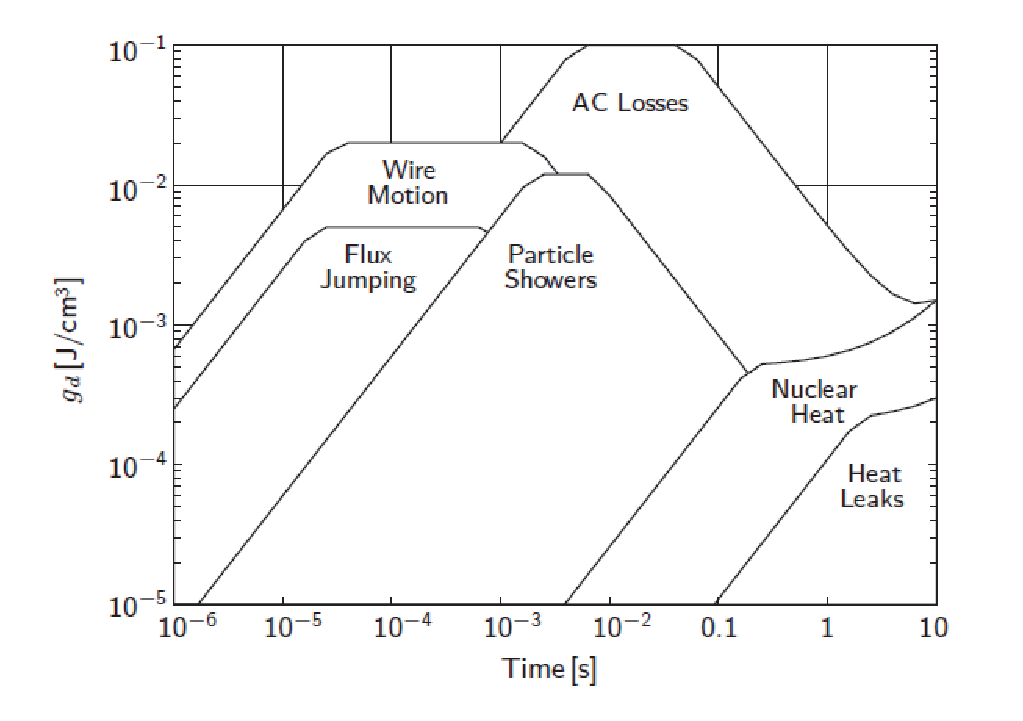
\includegraphics[scale=0.7]{chpt6/figs/fig6.1.eps}
	\caption{汇集的$g_d(t)$谱。}
\end{figure}

\subsection{稳定裕度 vs 扰动能}
所谓的``稳定裕度"或简单的``能量裕度"对绝热超导磁体是尤其有用的设计参数。
它就是载有运行电流$I_{op}(I_t)$的冷却或绝热的复合超导体所能吸收而又能维持全超导的
最大能量密度$\Delta e_h$。除非冷量可以平衡这个$\Delta e_h$,否则复合超导体将被加热,
其温度降上升至运行温度$T_{op}$之上;当它继续加热超导与$I_{op}$有关的``分享电流"温度$T_{cs}(I_{op})$
后,失去全超导。图6.2给出了第II类超导体临界电流与温度的关系$I_c(T)$,其中定义了$T_{cs}(I_{op})$。
$I_c(T)$近似是一条直线,连接了$T_{op}$下的临界电流$T_c(T_{op})\equiv I_{c_o}$以及$I_c(T_c)=0$。
实心原点定义$T_{cs}(I_{op})$为$I_c(T)$线和$I_{op}$对应的虚线的交点。
注意到$T_{cs}(I_{op})$是载有$I_{op}$的复合导体甚至在绝热条件下可以保持全超导的最高温度。
超过$T_{cs}(I_{op})$,基底常导金属开始``分享"电流,产生焦耳热耗散。
在绝热线圈中,从$T_{cs}(I_{op})$到临界温度$T_c$的转变差不多是瞬时的,在$T_c$及以上问题下,
基底材料载有差不多全部电流。
在图中还定义了$[\Delta T_{op}(I_{op})]_{st}=T_{cs}(I_{op})-T_{op}$,即复合导体从$T_{op}$
往上还能保持全超导所能承受的最大温度漂移极限。
有时候使用$[\Delta T_{op}(I_{op})]_{st}$而不是$\Delta e_h$来定量表示稳定性的程度。
在绝热条件下,$\Delta e_h$表示为: 
\begin{equation}% page357 第1个
\Delta e_h=\int_{T_{op}}^{T_{cs}(I_{op})}{C_{cd}(T)d(T)}=\int_{T_{op}}^{T_{op}+[\Delta T_{op}(I_{op})]_{st}}{C_{cd}(T)d(T)}
\end{equation}

注意到,$\Delta e_h$不仅依赖于$C_{cd}(T),T_{op}$和$T_{cs}(I_{op})$或$[\Delta T_{op}(I_{op})]_{st}$,
还依赖于与$I_{c_o}$有关的$I_{op}$($i_{op}\equiv I_{op}/I_{c_o}$)。
特别的,对于如图6.2这样的对$I_c(T)$的简单直线近似,$[\Delta T_{op}(I_{op})]_{st}$可由下式给出:
\begin{equation}% page357 第2个
[\Delta T_{op}(I_{op})]_{st}=(T_c-T_{op})(1-i_{op})
\end{equation}
\begin{figure}[htbp]
	\centering
	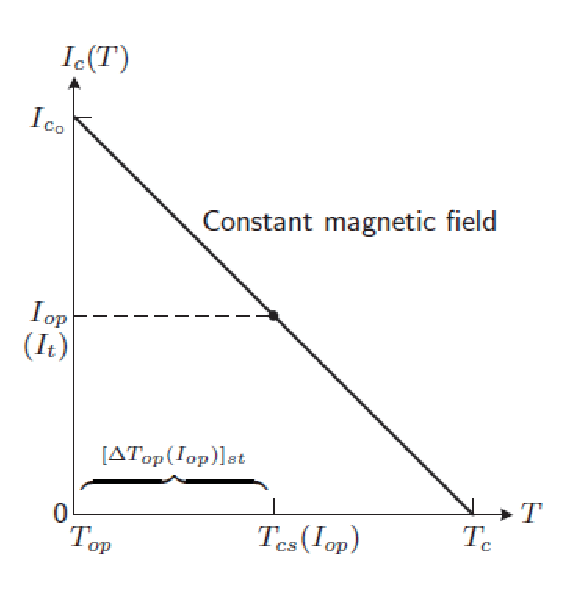
\includegraphics[scale=0.7]{chpt6/figs/fig6.2.eps}
	\caption{某第II类超导体的$I_c(T)$直线近似。}
\end{figure}

从方程6.3,我们可以得出,对一个绝热磁体,它的电流分享温度必须大于其运行温度($T_{cs}>T_{op}$),也即
它的$I_{op}(I_t)$应当在绕组中低于导体的最小$I_{c_o}$。因为$I_{c_o}$与磁场有关,而磁场在绕组中是变化的。
表6.4列出了几个对LTS和HTS磁体比较典型的$T_{op}$和$\Delta T_{op}$及其对应的$\Delta e_h$。

\begin{table}[htbp]\small
\centering
\caption{方程5.40在NbTi和YBCO材料的应用} 
\begin{tabular}{|c|c|c|c|c|c|}
\hline
\multicolumn{3}{|c|}{LTS} & \multicolumn{3}{c|}{HTS} \\ \hline
$T_{op}[K]$ & $[\Delta T_{op}(I_{op})]_{st}[K]$ & $\Delta
e_h[J/cm^3]$ & $T_{op}[K]$ & $[\Delta T_{op}I_{op}]_{st}[K]$
& $\Delta e_h[J/cm^3]$ \\ \hline
2.5 & 0.3 & $1.2\times10^{-4}$ & 4.2 & 25 & 1.6 \\
\hline
4.2. & 0.5 & $0.6\times10^{-3}$ & 10 & 20 & 1.8 \\
\hline
4.2 & 2 & $4.3\times10^{-3}$ & 30 & 10 & 3.7 \\
\hline
10 & 1 & $9\times10^{-3}$ & 70 & 5 & 8.1 \\
\hline
\end{tabular}
\end{table}


\begin{description}
	\item[LTS] 对比表6.4中给出的能量裕度与图6.1中给出的扰动能量密度,可以明确看到,LTS磁体非常容易因扰动
	而失超,失超对应的能量密度由方程6.1中的$g_d(t)$表示。为了应对这个情况,多年来人们一直进行技术开发以
	抑制这些扰动,如导线运动、磁通跳跃。对多数``直流"LTS绝热磁体,要最小化交流损耗以使其在大部分时间稳定运行。
	最小化或消除机械扰动(如导线运动)的技术仅对LTS磁体比较重要,第七章简要讨论。
	\item[HTS] 除了交流损耗,HTS磁体的扰动能量谱如图6.1所示。根据表6.4中的$\Delta e_h$,我们可以得出,HTS
	磁体至少在DC条件下,是绝对稳定的:于是,每一个DC HTS磁体都应被设计为绝热运行的。
\end{description}

\subsection{冷却}
尽管每一个超导磁体的运行都需要冷却,但如第四章论及,仅浸泡式低温稳定磁体需要\emph{在绕组间}用制冷剂冷却。
这样,方程6.1中的$-g_q(T)$项仅用于表示绕组内的冷却;绕组外的冷却,是每一个超导体都要求的,一般而言是外沿的;
它不出现于方程6.1中。
如上文讨论,HTS磁体能够,实际上也总是,绝热运行。此外,除了因耦合LTS磁体而运行于液氦温区的,多数HTS磁体都是
在$\sim$20 K以上运行。所以,液氦的传热数据对浸泡低温稳定HTS磁体设计不再是非常重要的;甚至液氮的传热数据
对HTS磁体也不是非常重要的,这是因为绝热运行时,绕组中根本没有液氮。

Bottura总结了氦在不同冷却区间的传热系数$h_q$与$\Delta T$的关系,如图6.3[6.14];这里的$\Delta T$一般是指
加热表面和4.2 K氦之间的温差。图中包括:1)核态沸腾和膜态沸腾,包括核态沸腾峰值点$h_{pk}=1.23\ \mathrm{W/cm^2 K}$;
2)暂态核沸腾;3)1.8 K(超流)和4.2 K下的Kapitza;4)3.5 atm和4.5 K下$10^4$和$10^5$两个雷诺数下的迫流。
这些图线中,包含峰值点的核态沸腾图是由浸泡式低温稳定磁体得出的;1.8 K的Kapitza图针对的是超流氦冷却的低温稳定磁体;
迫流图是针对的CICC绕成的低温稳定磁体。
\begin{figure}[htbp]
	\centering
	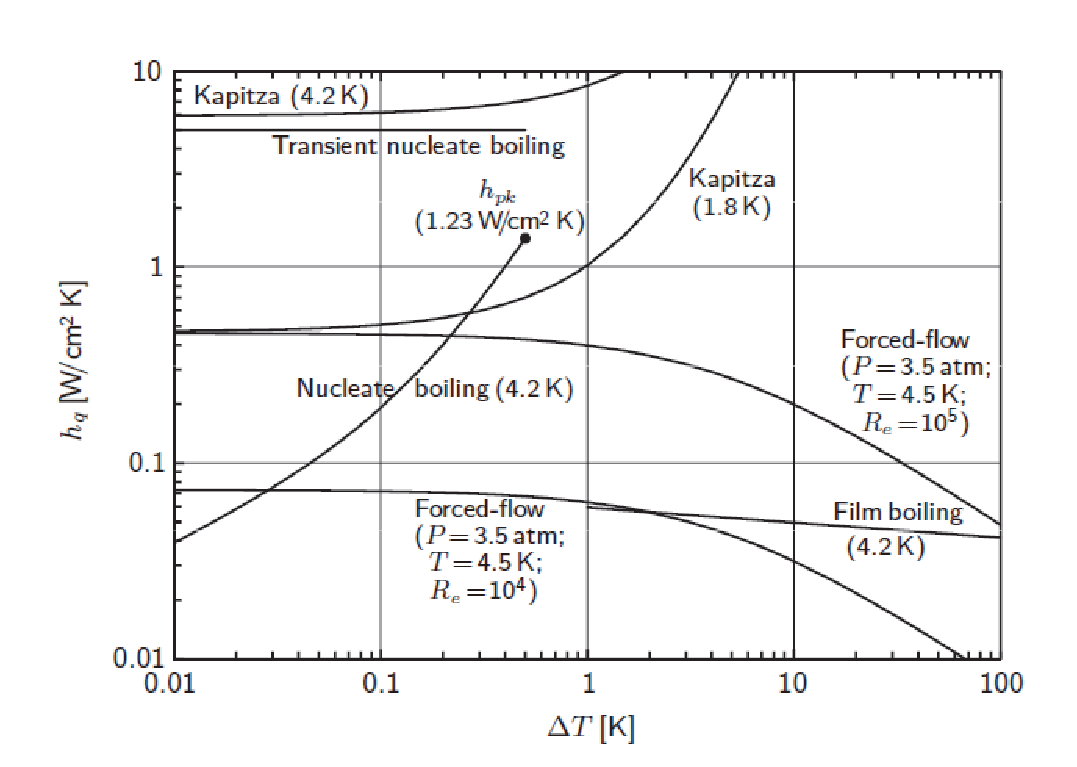
\includegraphics[scale=0.7]{chpt6/figs/fig6.3.eps}
	\caption{传热系数$h_q$与$\Delta T$的关系。}
\end{figure}

\section{电流密度}
磁体产生的磁场的计算中,一个关键参数是总电流密度$\lambda J$(方程3.108),它是由总安匝数$NI$除以磁体绕组截面积,
截面不仅包括载流导体,同时也包括绕组中的非载流部分。图6.4(a)给出了复合导体的截面积组成部分,图6.4(b)定义了整个
绕组的组成部分。两个图给出的是各部件代表性的常用组分。
\begin{figure}[htbp]
	\centering
	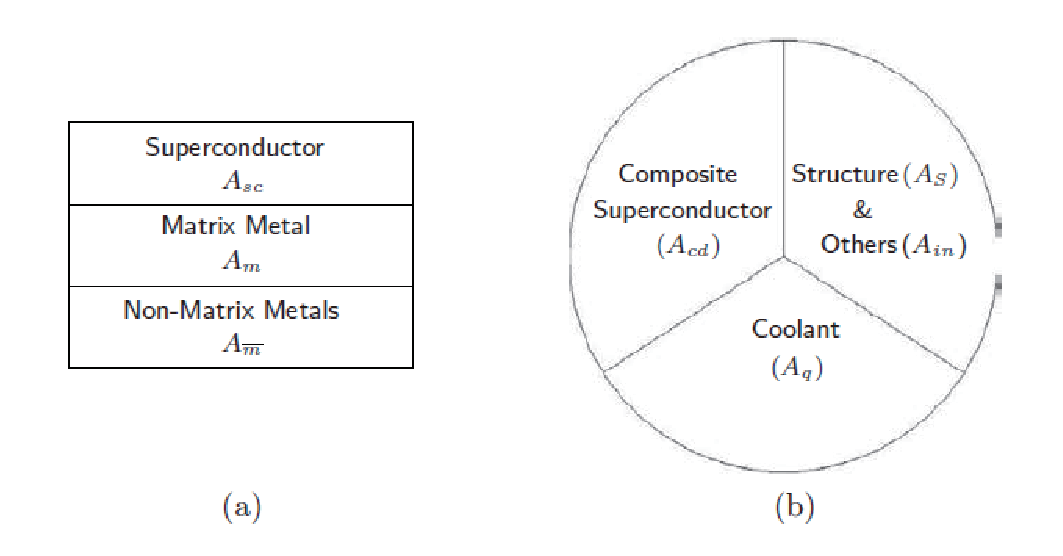
\includegraphics[scale=0.6]{chpt6/figs/fig6.4.eps}
	\caption{截面积的示意图:(a)复合导体;(b)全绕组。}
\end{figure}
\subsection{截面积}
如图6.4所示,超导体中至少有7个不同的截面积用于定义不同的电流密度:
图6.4a中对复合导体有$A_{sc},A_m$和$A_{\bar{m}}$;图6.4b中对全绕组有$A_{cd},A_s,A_{in}$和$A_q$。
$A_{\bar{m}}$,是非基底金属,在NbTi等合金中是0,但在$\mathrm{Nb_3 Sn}$和YBCO等化合物导体中不可忽略。
注意到,其他材料如绝缘体等占据的截面并未包括到总的超导体截面中来。
$A_S$通常是金属加强材料占据的截面,$A_{in}$包括绝缘体和有机填充材料如环氧等占据的截面。
除了下面将讨论的CICC导体,$A_S$和$A_{in}$通常可以统一归为结构部件。
复合导体和全绕组的总的截面积为:
\begin{subequations}
	\begin{align}
	A_{cd}&=A_{cs}+A_m+A_{\bar{m}}\\
	A_{wd}&=A_{cd}+A_S+A_{in}+A_q
	\end{align}
\end{subequations}

\subsection{复合超导体}
下面将定义并描述复合超导体的三个常用电流密度。

\textbf{超导体临界电流密度}

超导体临界电流密度$J_c$是由超导体在一定温度和磁场下的临界电流$I_c$除以截面$A_{sc}$(对NbTi和YBCO这种$A_{sc}$
可以明确量化的材料)或者$A_{sc}+A_{\bar(m)}$(对$\mathrm{Nb_3 sN}$这样非基底金属是一个联合部分的材料)得到的:
\begin{subequations}
	\begin{align}
	J_c&\equiv\frac{I_c}{A_{sc}}\\
	J_c&\equiv\frac{I_c}{A_{sc}+A_{\bar{m}}}
	\end{align}
\end{subequations}

在材料发展阶段中(表1.4中的阶段1),定义为$J_c\equiv I_c/A{sc}$的$J_c$以及$H_{c2}$和$T_c$是描绘超导体性能
的最合适、最有用的参数。

\textbf{工程(或导体)临界\& 运行电流密度}

工程(或导体)临界\& 运行电流密度$J_e (J_{cd})$考虑了工艺和磁体需求。$A_{\bar{m}}$和$A_m$都是磁体级别超导体
的关键参数:
\begin{equation}% page360 第5个
J_e=J_{cd}\equiv\frac{I_c}{A_{cd}}=\frac{I_c}{A_{sc}+A_m+A_{\bar{m}}}
\end{equation}

在CICC导体(讨论6.6)中,结构组分$A_S$和制冷工质组分$A_q$的截面也是导体的组成部分,所以他们也常被包含到$A_{cd}$
中去。当导体运行于电流$I_{op}$时,我们还可以定义工程(或导体)运行电流密度:$J_{e_o}=J_{cd_o}\equiv I_{op}/A_{cd}$。
$J_{cd_o}(t)$隐含了$I_{op}(t)$可随时间变化。

\textbf{基底电流密度}

基底电流密度$J_m$对由复合导体绕成的磁体的稳定性和保护是一个非常重要的参数。$J_m$定义为通过基底的电流除以其截面积。
\begin{equation}% page361 第1个
J_{m}\equiv\frac{I_m}{A_m}    \ \mbox{or}\    J_m(t)\equiv\frac{I_m(t)}{A_m}
\end{equation}

其中,$I_m$是运行(传输)电流$I_{op}(I_t)$的一部分或全部,而$I_{op}(I_t)$取决于超导体是否超导。
\begin{align*}% page361 第2个
I_{op}=I_t=I_m+I_s  \ \mbox{or}\ I_{op}(t)=I_{t}(t)=I_m(t)+I_s(t) \tag{6.7b}
\end{align*}

式中,$I_s$是通过超导体的电流。因为最相关的基底电流就是正常运行电流$I_{op}$,所以当$I_s=0$时,
常用另一个基于$I_{op}$的基底电流密度:
\begin{align*}% page361 第3个
J_{m_o}\equiv I_{op}   \ \mbox{or}\  J_{m_o}(t)\equiv\frac{I_{op}(t)}{A_m} \tag{6.7c}
\end{align*}

\subsection{绕组中的电流密度}
由第三章的研究以及上面简要的概述,我们知道磁体产生的磁场直接正比于磁体绕组的全电流密度。
我们可以使用两个电流定义这个电流,一个是表示任意电流的$I$,另一个是表示磁体运行电流的$I_{op}$:
\begin{subequations}
	\begin{align}
	\lambda J&\equiv\frac{I}{A_{wd}}\\
	\lambda J_{op}\equiv\frac{I_op}{A_{wd}}&  \ \mbox{or}\  \lambda J_{op}(t)\equiv\frac{I_{op}(t)}{A_{wd}}
	\end{align}
\end{subequations}

因为在这里讨论的所有电流密度中,是$\lambda J_{op}$决定了磁体产生的场,所以它对磁体费用的影响最为直接。
因此,对一个在市场中有竞争力的磁体而言,$\lambda J_{op}$必须尽可能的大,当然也需要考虑具体的磁体的设计、运行需要。
(第三章中,为了简单起见,$\lambda J_{op}$由$\lambda J$取代了。)

\textbf{CICC导体的电流密度}

CICC导体,用于大型和高场磁体(将在讨论6.6详细描述)。
因为在CICC中,导体和绕组是耦合的,我们需要特别定义一个导体电流密度$J_{cic_o}$,描述运行电流下的CICC导体:
\begin{subequations}
	\begin{align}
	J_{cic_o}\equiv\frac{I_{op}}{A_{cic}}\ \mbox{or}\ J_{cic_o}\equiv\frac{I_{op}(t)}{A_{cic}}\\
	A_{cic}\equiv A_{cd}+A_S+A_q
	\end{align}
\end{subequations}


\section{专题}
\subsection{讨论6.1:低温稳定性---电路模型}
此处我们讨论低温稳定性的理论。我们采用电路模型来研究由超导体嵌入铜基底而组成的复合导体的行为。

图6.5a给出了超导体的理想$R_s$和$I$关系图,其中,$R_s$是超导体的电阻---这个图可用于多数LTS,
而对多数HTS不适用。此处所谓的理想,是指在$I_s<I_c$时,$R_s=0$,其中$I_c$是超导体的临界电流。
在$I_s>I_c$时,$R_s=R_n$,其中,$R_n$是超导体在正常态的电阻;在$I_s=I_c$时,$0\le R_s\le 	R_n$,
也即它满足电路条件。图6.5b给出了在温度$T$下载有传输电流$I_t$的复合超导体的电路模型。
$I_s$是通过超导体的电流,$R_m$是基底金属的电阻;一般有$R_m\ll R_n$。

\textbf{$I_t\le I_c$区}\quad 此时,超导体载有全部传输电流,$I_s=I_t\le I_c$。由图6.5a有$R_s=0$,
由图6.5b有$V_{cd}=0$,其中$V_{cd}$是复合导体上的电压。总焦耳热耗散$G_j$为零。

\textbf{$I_t>I_c$区}\quad 当$I_t>I_c$,由于$R_m\ll R_n$,超过$I_c$的电流几乎都将流过铜基底。
也即。$I_m\simeq I_t-I_c$以及$I_s\simeq I_c$。其中,$I_m$是通过基底的电流。于是:
\begin{subequations}
	\begin{align}
	V_{cd}&=R_mI_m\simeq R_m{(I_t-Ic)}\\
	G_{j}&=V_{cd}I_t
	\end{align}
\end{subequations}

联立上面两个方程,有:
\begin{equation}% page362 第3个 6.11
{(G_j)}\simeq R_{m}I_{t}{(I_t-I_c)}
\end{equation}

注意,$G_j$与温度无关,和$R_m,I_c$一样。因为基底金属(如铜)的电阻在4-30 K范围内几乎与温度无关,
$R_m$在LTS的稳定性分析时,总是假定为常数。
\begin{figure}[htbp]
	\centering
	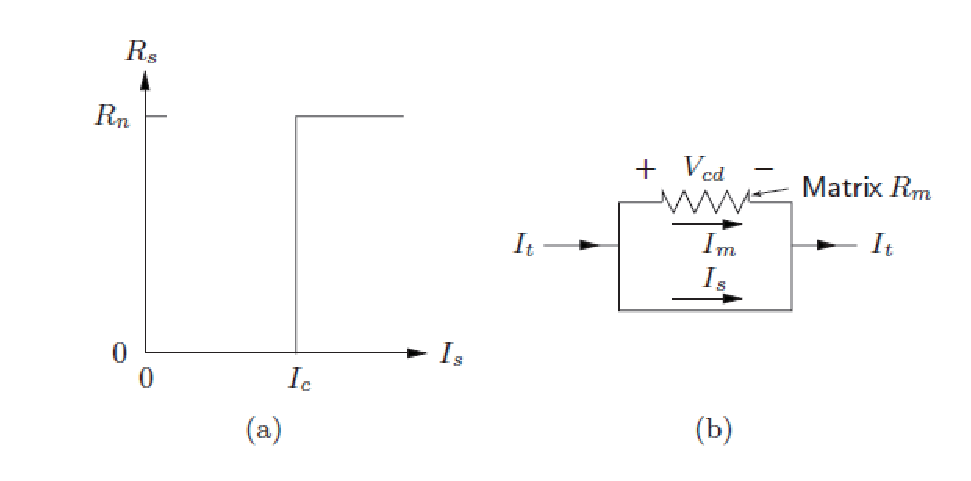
\includegraphics[scale=0.7]{chpt6/figs/fig6.5.eps}
	\caption{(a)超导细丝$R_s$和$I$关系图;(b)复合超导体的电路模型。}
\end{figure}

\subsection{问题6.1:低温稳定性---温度依赖}
下面我们考察复合导体单位长度总焦耳热耗散$G_j$对温度的依赖关系(讨论6.1中的方程6.11)。
图6.6(与图6.2相同)给出了$I_c$与$T$的关系,该关系常用于近似超导体在恒定磁场下的$I_c(T)$
(方程5.38给出了临界电流密度的相同的线性近似)。
注意到$I_c(T_{op})=I_{c_o},\ I_c(T_c)=0$。当温度变化时,通过复合导体的净传输电流$I_t$仍保持不变。
电流分享温度$T_{cs}$如图,有$I_t=I_c(T_{cs})$给出。

a) 超导体的$I_c(T)$由下式近似:
\begin{equation}% page363 第1个 6.12
I_c(T)=I_{c_o}(\frac{T_c-T}{T_c-T_{o_p}}) (T_{o_p}\leq T \leq T_c)
\end{equation}

证明,$G_j$有如下的温度依赖关系:
\begin{subequations}
	\begin{align}
	G_j(T)&=0 &(T_{o_p}\leq T \leq T_{cs})\\
	G_j(T)&=R_mI_t^2(\frac{T-T_{cs}}{T_c-T_{cs}})&(T_{cs}\leq T\leq T_c)\\
	G_j(T)&=R_mI_t^2 &(T\ge T_c)
	\end{align}
\end{subequations}
假定$R_m$与温度无关。

b) 画出从$T_{op}$到$T>T_c$温度范围的方程6.13的关系图。

c) 给出方程6.13b给出的$G_j$的物理解释。

d) 定性的讨论方程6.13b如何在30 K以上修正。30 K之上,$R_m$将依赖于温度,成为$R_m(T)$,这是复合HTS的情况。

\begin{figure}[htbp]
	\centering
	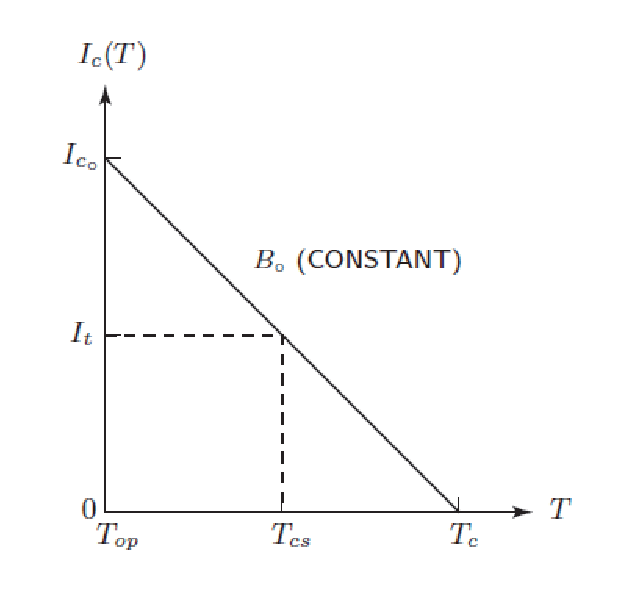
\includegraphics[scale=0.7]{chpt6/figs/fig6.6.eps}
	\caption{超导体的$I_c(T)$线性近似。}
\end{figure}

\subsubsection{问题6.1之解}
a) 因为$T_{op}\le T\le T_{cs}$时,有$I_c(T)>I_t$(图6.6),我们有:
\begin{align*}
G_j(T)=0 \quad (T_{o_p}\leq T \leq T_{cs}) \tag{6.13a}
\end{align*}

将6.12给出的$I_c(T)$代入6.11给出的$G_j$中,有
\begin{align*}
G_j(T)&=R_m I_t[I_t-I_{c_o} \left(\frac{T_c-T}{T_c-T_{op}}\right)]\quad (T_{cs}\leq T\leq T_c) \tag{S1.1}
\end{align*}

令$I_t=I_c(T_{cs})$,并将之代入6.12,有:
\begin{align*}% page364 第3个 S1.2
I_{c_o}=I_t\left(\frac{T_c-T_{op} }{T_c-T_{cs}}\right) \tag{S1.2}
\end{align*}

式中,$I_{c_o}\equiv I_c(T_{op})$。联立S1.1和S1.2,有:

\begin{align*}
	G_j(T)=R_mI_t^2(\frac{T-T_{cs}}{T_c-T_{cs}}) (T_{cs}\leq T\leq T_c) \tag{6.13b}
\end{align*}
\begin{align*}
    G_j(T)=R_mI_t^2 (T\ge T_c) \tag{6.13c}
\end{align*}


b) 如图6.7。
\begin{figure}[htbp]
	\centering
	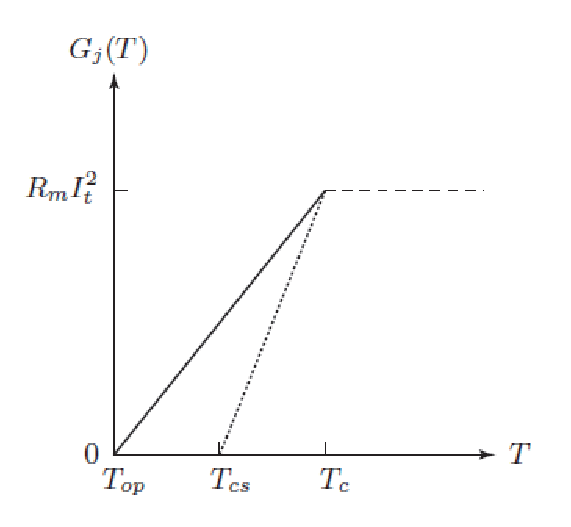
\includegraphics[scale=0.7]{chpt6/figs/fig6.7.eps}
	\caption{复合导体的$G_j(T)$图,其中$R_m$为常数。}
\end{figure}

c) 明显,只要$I_t<I_c(T)$,所有的传输电流都只通过超导体,$V_{cd}=0$,故$G_j(T)=0$。
在电流分享温度$T_{cs}$下,当$I_t=I_c$时,超导体载有其为超导态下的最大可能电流;在$T_{cs}$之上,
电流开始向铜基底分流,在复合导体内产生焦耳热。
随着$T$升高,这个分流持续增加,直到达到$T_c$,在这个点几乎全部传输电流都被转移至基底中,
当然其假设是$R_m\ll R_n$,而它通常是合理的。因为$R_m$是常数,所以$G_j$在温度$T_{cs}$和$T_c$
之间随$T$的变化时线性的。$R_m$是常数这个假设对多数基底金属(如铜)在$T_{op}$小于30 K时都是有效的。

d) 如果$T_{op}>\sim 30$ K,$R_m$的常数假设就不合理的。也即,对多数HTS,应将其做温度依赖看待。
方程6.13b和6.13c相应的修正为:
\begin{subequations}
	\begin{align}
	T_{cs}\leq T\leq T_c:\quad G_j(T)&=R_m(T)I_t^2(\frac{T-T_{cs}}{T_c-T_{cs}})\\
	T\ge T_c:\quad G_j(T)&=R_m(T)I_t^2
	\end{align}
\end{subequations}


\subsection{讨论6.2:Stekly低温稳定性判据}
在6.2.1节,我们看到所谓的Stekly低温稳定性判据通过浸泡到绕组中去的制冷剂平衡了复合超导体产生的焦耳热。
这样,方程6.1可以化简为:
\begin{equation}% page365 第1个 6.15
C_{cd}(T)\frac {\partial T}{\partial t}=\nabla\cdot[k_{cd}(T)\nabla T]+\rho _{cd}(T)J_{cd}^2(t)+g_d(t)-(\frac{f_p\ \mathrm{P}_D}{A_{cd}})g_q(T)
\end{equation}

式中,等号左侧、等号右侧第一项、第三项可以忽略。
式中,$P_D$是从的导体周长;常数$f_D$是置于制冷剂中的$P_D$分数。
Stekly首先通过选择$I_t=I_{c_o}$(令$I_t$等于超导体在$T_{op}$下的临界电流)发展了他的理论。
注意到,$I_t$还表示运行电流$I_{op}$,那么选择$I_t=I_{op}=I_{c_o}$使得$T_{cs}=T_{op}$,
以及6.13b成为:
\begin{subequations}
	\begin{align}
	G_j(T)&=R_mI_{c_o}^2(\frac{T-T_{op}}{T_c-T_{op}}) &(T_{o_p}\leq T \leq T_c)\\
	\rho_{cd}J^2_{cd}(t)&=\frac{\rho_{m}I_{co}^2}{A_{cd}A_m}
	(\frac{T-T_{op}}{T_c-T_{op}}) &(T_{o_p}\leq T \leq T_c)
	\end{align}
\end{subequations}

历史上,Stekly选择$I_t=I_{c_o}$发展他的判据不是为了超导磁体的稳定性,而是为了解释
在V-I测试时超导体测试样品在其电流超过$I_{c_o}$后的分流。
现在,每一个LTS超导磁体的运行电流都选在小于$I_{c_o}$。对于HTS磁体,稳定性不是重要的设计问题;
但是类似LTS测试样品,HTS测试样品也存在稳定性问题。
V-I特性相关的稳定性问题将在问题6.5中研究。

Stekly的冷却选择是温度线性的:
\begin{equation}% page365 第3个 6.17
g_q(T)=h_q(T-T_b)\simeq h_q(T-T_{op})
\end{equation}

式中,$T$是导体的表面问题。$T_b$是冷池(制冷剂)的问题,假定其等于$T_{op}:T_b\simeq T_{op}$。

根据6.15,Stekly低温稳定性判据要求$(f_p P_D/A_{cd})g_q(T)\ge \rho_{cd}(T)J_{cd}^2(t)$。
根据6.16b和6.17,我们有:
\begin{equation*}% page365 第4个 6.18
\frac{f_pP_Dh_q(T-T_{op}}{A_cd}\geq \frac{\rho_m I_{co}^2}{A_{cd}A_m}(\frac{T-T_{op}}{T_c-T_{op}})
\end{equation*}
\begin{equation}% page365 第4个 6.18
\frac{\rho_m I_{co}^2}{f_pP_DA_mh_q(T_c-T_{op})}\leq 1
\end{equation}

Stekly稳定性参数$\alpha_{sk}$由6.18给出:
\begin{equation}% page365 第5个 6.19
\alpha_{sk}=\frac{\rho_m I_{co}^2}{f_pP_DA_mh_q(T_c-T_{op})}
\end{equation}

注意到,无量纲参数$\alpha_{sk}$表示的是焦耳耗散密度和冷却功率的比值。于是,当$\alpha_{sk}\le 1$
时(冷量足够),运行时稳定的;当$\alpha_{sk}> 1$时(冷量不够)不稳定。

根据Stekly稳定性判据,1960年代和1970年代建造和可靠运行的多数大型磁体都是低温稳定的。
方程6.19表明$\alpha_{sk}\propto 1/A_m$,即对给定的冷却条件,稳定性或可靠性与$A_m$有直接关系。反过来:
\begin{equation}% page366 第1个 6.20
A_m=\frac {\rho_mI_{co}^2}{\alpha_{sk}f_pP_Dh_q(T_c-T_{op})}
\end{equation}

为了在给定冷却条件下实现更大程度的稳定性,在浸泡冷却的低温稳定磁体中,增加$A_m$十分必要。
复合超导体在运行电流下的电流密度$J_{op}$为:
\begin{align*}% page366 第2个 6.6
J_{op}=\frac{I_{op}}{A_{sc}+A_ {\bar{m}}+A_m}\tag{6.6}
\end{align*}
\begin{equation}% page366 第2个 6.21a
=(\frac{\gamma_{m/s}}{\gamma_{m/s}+1})J_{m_0}
\end{equation}

式中的面积比$\gamma_{m/s}$定义为:
\begin{align*}% page366 第3个 6.21b
\gamma_{m/s}\equiv \frac{A_m}{A_{sc}+A_m}
\end{align*}

在NbTi中,$\gamma_{m/s}$被称为基底-超导体比率,在$\mathrm{Nb_3Sn}$中称为基底-非基底比率。
显然,当$\gamma_{m/s}\gg 1$时,有$J_{op}\simeq J_m$。

很明显,在这些早期的大型磁体中,稳定性无疑是优先于效率考虑的。这种哲学一直持续到今天,
特别大型磁体。而大型磁体中,还有另一个可能比稳定性更重要的问题需要考虑:电磁力。
大型低温稳定LTS磁体要求的加强组件$A_S$在限制绕组的总电流密度上,比基底金属$A_m$更重要。

表6.5列出了两个低温稳定LTS磁体(一个是1960年代末期的NbTi磁体,一个是近期的CIC $\mathrm{Nb_3Sn}$磁体)的电流参数---$I_c,I_{op},\gamma_{m/s},J_c(=I_c/A_{sc}),J_e(=I_c/A_{cd}),
J_{m_o}(=I_{op}/A_m),\lambda J_{op}(=I_{op}/A_{wd})$[6.12,3.24]。
相比于NbTi磁体,$\mathrm{Nb_3Sn}$磁体的$\gamma_{m/s}$更小,这意味着它的$\lambda J_{op}$更好。
这个性能的提高部分是由于近四十年来随着建造实际磁体而逐步深入的对稳定性和保护问题的理解,
部分来自降低这种仅用于研究的个性化磁体的费用的压力。

\begin{table}[]
\begin{tabular}{|c|c|c|c|c|c|c|c|}
\hline
Composite & $\gamma_{m/s}$    & $I_c[KA]$    & $I_{op}[KA]$    &
$J_c[MA/m^2]$   & $J_e[MA/m^2]$    & $J_{mo}[MA/m^2]$   & $\lambda
J_{op}[MA/m^2]$    \\ \hline
$NbTi^*$      & 24   & $4.0^{a}$  & 2.2  & 800 & 32.0 & 18.3 & 7.8  \\
\hline
$NbSn\dag $     & 21.5 &$ 15.8^{b} $& 10.0 & $627^{c}$ & 74.4 & 184  &
39.2 \\ \hline
\end{tabular}
\end{table}


\begin{table}[htbp]\small
\centering
\caption{方程5.40在NbTi和YBCO材料的应用}  %6.5
\begin{tabular}{|c|c|c|c|c|c|c|}
\hline
 $I_t[A]$   &$I_m[A]$         &$I_s$[A]          &$R_mI_m[V]$
 &$P_{cd}[W]$      &  $g_{jcd}[W/cm^2]$    & $R_{dif}[\Omega]$      \\
 \hline
90  & 0.00686 & 89.99314 & 2.06$\times10^{-6}$ & 185$\times10^{-6}$  & 18.5$\times10^{-6}$ & 0.343$\times10^{-6}$ \\ \hline
100 & 0.0332  & 99.967   & 9.95$\times10^{-6}$ & 995$\times10^{-6}$  & 99.5$\times10^{-6}$ & 1.49$\times10^{-6}$  \\ \hline
120 & 0.483   & 119.517  & 145$\times10^{-6}$  & 17.4$\times10^{-3}$ & 1.74$\times10^{-3}$ & 18.2$\times10^{-6}$  \\ \hline
150 & 7.07    & 142.93   & 2.12$\times10^{-3}$ & 318$\times10^{-3}$  & 31.8$\times10^{-3}$ & 223 $\times10^{-6}$  \\ \hline
300 & 126.75  & 173.25   & 38.0$\times10^{-3}$ & 11.4 & 1.14 & 3.29$\times10^{-3}$  \\ \hline
500 & 315.88  & 184.12   & 94.8$\times10^{-3}$ & 47.4 & 4.74 & 7.72$\times10^{-3}$  \\ \hline
\end{tabular}
\end{table}




\subsection{讨论6.3:复合物超导体}
可用的磁体级超导体通常有两类,一类是``Monolithic"(单体),一类是``built-up"(组合)。

\textbf{A. Monolith}

超导体和正常金属通过简单合金工艺形成一个实体。视觉上看,除了在导体截面上,不能分辨出一个一个单体上存在
多与一种组分。多数圆线复合导体都是单体的。尽管$\gamma_{m/s}$值大于10,但在合金过程中不折断
细丝而生成单体超导体很难,特别是那些细丝直径小于100 $\mu$m的尤其难。

\textbf{B. Build-up}

组合的超导体由$\gamma_{m/s}$接近1的单体超导体和正常金属稳定部分组成,金属稳定部分通常是焊在
处理后的单体上的。稳定部分的机械性能因而不受到单体处理过程的影响,从而能更容易满足导体规格要求。
CIC导体是一种组合导体变种。

\subsection{问题6.2:低温稳定性---非线性冷却曲线}
讨论6.2推出的参数$\alpha_{sk}$是基于与温度无关的传热系数$h_q$的。
实际中,冷却曲线,甚至低温稳定磁体通畅运行的核态沸腾传热区域都是非线性很严重的,一个例子如图4.1所示。
于是,直接从低温稳定性判据导出热流曲线$q(T)[\mathrm{W/cm^2\ or\ W/m^2}] $。

a) 证明$I_{op}$下的基底电流密度$[J_{m_o}]_{sk}$满足Stekly低温稳定性判据的一个变体,
该变体结合了热流密度曲线$q(T)$:
\begin{equation}% page367 第1个 6.22
[J_{m_o}]_{sk}=\sqrt{\frac{f_pP_Dq_{fm}}{\rho_mA_m}}
\end{equation}

式中,$q_{fm}$是膜态沸腾区域的最小热流密度。

b) 在$I_{op}=I_{c_o}$时,在同一个图中定性画出$q(T)$曲线和尺度一致的产热曲线,并在图中指出稳定运行的区域。
其中,$I_{c_o}$是超导体在$T_{op}$时的$I_c$。

c) 在b)的同一个图上推广b)到$I_{op}<I_{c_o}$的情况。证明,在这个条件下,电流分享温区的
$g_j(T_c)$和$d\hat{g}_j(T)/dT$小于$I_{op}=I_{c_o}$条件下的。

\subsubsection{问题6.2之解}
a) 在应用低温稳定性的多数应用中,我们必须假定超导体可能运行在完全正常态。然后,选择膜态沸腾区域的最小热流
是最安全的。于是:
\begin{align*}% page368 第1个 S2.1
\frac {\rho_mI_{co}^2}{A_m}=f_pP_Dq_{fm} \tag{S2.1}
\end{align*}

解出$[J_{m_o}]_{sk}$,得到:
\begin{align*}% page368 第2个 6.22
[J_{m_o}]_{sk}=\sqrt{\frac{f_pP_Dq_{fm}}{\rho_mA_m}} \tag{6.22}
\end{align*}

b) 图6.8给出了液氦$q(T)$的典型曲线。图中同时还画出了$\hat{g}_j(T)\equiv (A_{cd}/f_p P_D)g_j(T)$曲线。
通过选择合适的参数,$\hat{g}_j(T)\equiv (A_{cd}/f_p P_D)g_j(T)$略小于$q_{fm}$。

c) 图6.8中的虚线表示$I_t<I_{c_o}$的情况。在温区$T_{op}\le T\le T_{cs}$,导体是全超导的。
因为$G_j(T_{op})=R_m I_t^2$,很明显,它在$I_t<I_{c_o}$时更小。根据问题6.2的S1.2:
\begin{align*}% page368 第3个 s1.2
I_{c_o}=I_t(\frac{T_c-T_{op} }{T_c-T_{cs}}) \tag{S1.2}
\end{align*}

联立S1.2和6.13b,有:
\begin{align*}% page368 第4个
g_j(T)&=(\frac{A_{cd}}{f_pP_D})R_mI_t^2=(\frac{A_{cd}}{f_pP_D})R_mI_{co}^2\frac{(T_c-T_{cs})^2(T-T_{cs})}{(T_c-T_{op})^3}\\
\frac{dg_j(T)}{dT}&=(\frac{A_{cd}}{f_pP_D})R_mI_{co}^2\frac{(T_c-T_{cs})^2}{(T_c-T_{op})^3}
\end{align*}

这样,$G_j(T_{op})$在$I_t=I_{c_o}(T_{cs}=T_{op})$时就要大于$I_t<I_{c_o}(T_{cs}>T_{op})$对应的值了。
\begin{figure}[htbp]
	\centering
	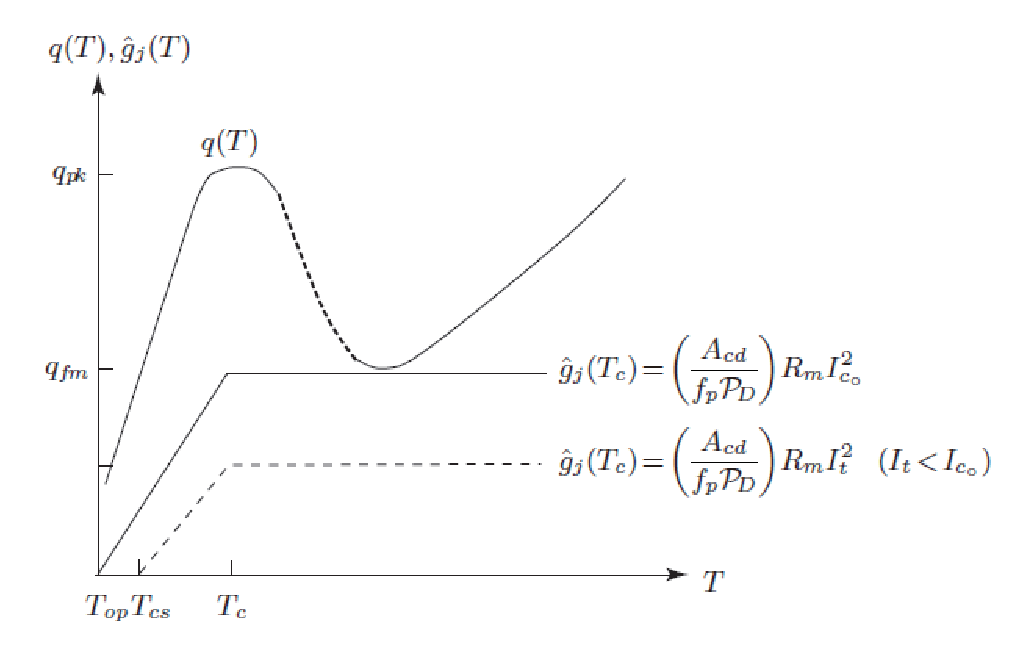
\includegraphics[scale=0.7]{chpt6/figs/fig6.8.eps}
	\caption{液氦$q(T)$的定性图,以及$I_{op}=I_{c_o}$(实线)和$I_{op}<I_{c_o}$(虚线)$两种情况下的$$\hat{g}_j(T)$图。}
\end{figure}


\subsection{讨论6.4:``等面积"判据}
Maddock、James和Norris的等面积判据[6.15]是低温稳定性判据的一个变体,保留了方程6.1中的热传导项。
于是,等面积判据仅在焦耳热耗散不再整个绕组内全局扩散的条件下成立。
在Stekly低温稳定性判据中,焦耳热耗散是局域的,且完全被冷却项$g_q(T)$平衡掉;在等面积判据中,
导体轴向的热传导起到移除当地焦耳热的辅助作用。
因为判据应用于浸泡低温冷却磁体,它主要用于液氦冷却的LTS磁体。
等面积判据要求满足下面的条件:
\begin{equation}% page369 第1个 6.23
\int_{T_{op}}^{T_{eq}}[g_q(T)-(\frac{A_{cd}}{f_pP_D})g_j(T)]d(T)
=\int_{T_{op}}^{T_{eq}}[g_q(T)-\hat{g}_j(T)]dT=0
\end{equation}

式中,$T_{eq}$是高于$T_{op}$的温度,在该温度下有$g_q(T)=\hat{q}_j(T)$。
$g_q(T)$是对流热流;$g_i(T)$是焦耳热耗散密度,可由方程6.13的$G_j$经代入
$T_{cs}=T_{op}$(在$T_{cs}>T_{op}$时,使用6.14式)和$J_{m_o}=I_{op}/A_m$得到:
\begin{subequations}
	\begin{align}
	g_j(T)&=\rho_m(T)J_{m_o}^2(\frac{T-T_{op}}{T_c-T_{op}}) &(T_{op}\leq T \leq T_c)\\
	g_j(T)&=\rho_m(T)J_{m_o}^2 &(T \geq T_c)
	\end{align}
\end{subequations}

图6.9给出了$\hat{q}_j(T)$曲线的一个满足等面积判据的例子。
本例中,方程6.23通过令图6.9中两个交叉线区域相等而满足。
物理上看,在温度为$\sim T_c$至$T_{eq}$``较热"区域中``多出"的热被传导至温度
为$T_{op}$至$\sim T_{c}$的``较冷"区域;较冷区域提供了``多出"的冷量。
从图6.9可明显看出,相比Stekly低温稳定性判据,
复合超导体的焦耳热耗散线$\hat{g}_j(T\ge T_c)$能更好的满足等面积判据。
\begin{figure}[htbp]
	\centering
	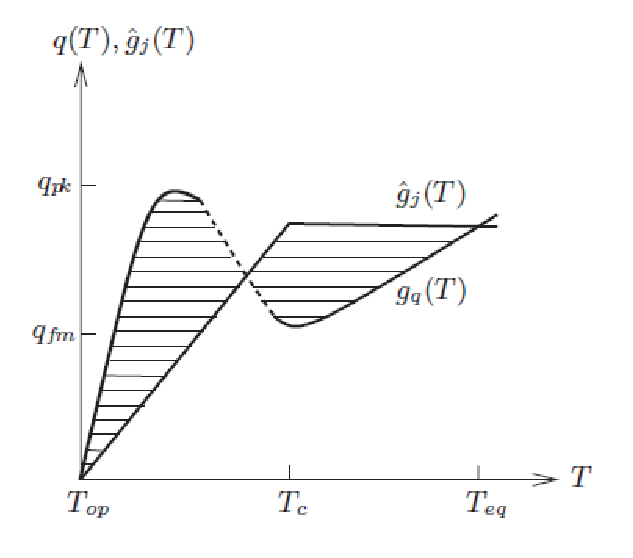
\includegraphics[scale=0.7]{chpt6/figs/fig6.9.eps}
	\caption{满足等面积判据的$\hat{q}_j(T)$曲线例子。}
\end{figure}

Wislon将这个1D等面积判据扩展到2D等面积判据[6.16];
2D判据已经饼式测试线圈实验验证。

\subsection{讨论6.5:超导体``指数"n}
超导体的``实际"和``理想"电压-电流特征曲线可由下面的``唯象"关系刻画:
\begin{equation}% page370 第1个 6.25a
V_s=V_c(\frac{I_s}{I_c})^n
\end{equation}

式中,$V_s$和$I_s$分别是超导体的电压(单位轴向长度)和电流;$I_c$是特定判据电压$V_s$下的临界电流;
$n$是超导体指数。方程6.25也可由超导体的电场和电流密度表达:
\begin{align*}% page370 第2个 6.25b
E_s=E_c(\frac{I_s}{I_c})^n \tag{6.25'}
\end{align*}

很明显,$E_c$代表一个特定的临界电场,HTS通常是$1\times 10^{-4}$ V/m,而LTS一般要小1到2个数量级。

一个理想的超导体,即在$I_c$下零点阻对应$n=\infty$。
在磁体级超导体中,实际且有潜力的如NbTi、$\mathrm{Nb_3 Sn}$、Bi2223、Bi2212和图层YBCO,LTS的
$n$值通常在$\sim$30至$\sim$80;HTS的在$\sim$10到$\sim$40.

就如开始所述,方程6.25(或6.25')是唯象的。
它是简单的基于实验V-I数据得到的:$n$是通过在$I_s$附近你和$V_s$和$I_s$数据得到的。
预测$n$值没有任何理论基础,尽管非均匀细丝直径这样的低质量超导体确是低$n$值的原因[6.17]。
因为实操中测量低于$\sim 0.8 I_c$下的$V_s$---纳伏或更小---很困难,检验6.25在$\sim 0.8 I_c$下的有效性
也就很困难[6.18]。HTS的指数问题已有研究[6.19],结果已用于YBCO线圈的设计[6.20]。

图6.10给出了基于6.25在$n_1=5,n_2=50,n_3=\infty$等3个指数下的$V_s$ vs. $I_s$关系图以及判据电压下的
临界电流。所以,图6.5的$R_s$ vs. $I_s$图对应理想超导体。
\begin{figure}[htbp]
	\centering
	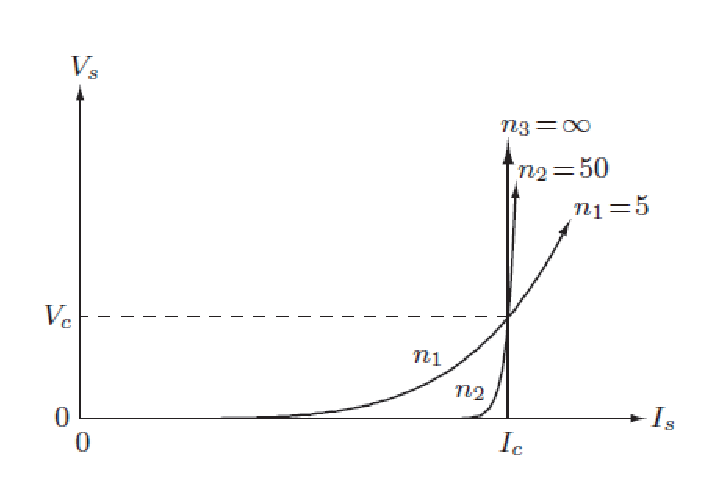
\includegraphics[scale=0.7]{chpt6/figs/fig6.10.eps}
	\caption{在$n_1=5,n_2=50,n_3=\infty$等3个指数下的$V_s$ vs. $I_s$关系图以及判据电压下的
		临界电流。}
\end{figure}

\subsection{问题6.3:复合物超导体(n)---电路模型}
对复合超导体,其超导特性可由6.25描写的,图6.5b的等效模型经修正如图6.11。
它由一个理想电压源(无内阻)$V_S$串联一个差分电阻($R_{dif}\equiv \partial V_s/\partial I_s$,$V_s$是跨越超导体的电压)而成。如图6.5b一样,基底由电阻$R_m$代表。

a) 证明,在$R_c\equiv V_c/I_c$时,$R_s\equiv V_s/I_s$和$R_{dif}$为:
\begin{subequations}
	\begin{align}
	R_s&=R_c(\frac{I_s}{I_c})^{(n-1)}\\
	R_{dif}&=nR_c(\frac{I_s}{I_c})^{(n-1)}
	\end{align}
\end{subequations}

可见,$R_{dif}=nR_s$。对于$n=1$的超导体,其V-I曲线类似于常规电阻,有$R_s=R_c=R_{dif}$。

b) 对一条10 cm长、1 cm宽的复合超导体,在77.3 K时$I_c=100$ A,$V_c=10\ \mu$V,$n=15$,
基底电阻$R_m=0.3\ \mathrm{m}\Omega$。出于简单性,假设复合导体由维持77.3 K的沸腾液氮冷却, 
计算:1) $I_m$和$I_s$;2)跨越10 cm长复合导体的总电压;3)复合导体内的总焦耳热;4)冷却表面
为$10\ \mathrm{cm^2}$下的焦耳热密度;5)在传输电流$I_t$为90A、100A、120A、150A、300A和500A
时的$R_{dif}$。

c) 讨论恒温77.3 K假设,定性讨论如果复合导体的温度随着焦耳热增加而升高,结果如何修正?

d) 令$n=30$,重复b)。

e) 令$n=60$,重复b)。
\begin{figure}[htbp]
	\centering
	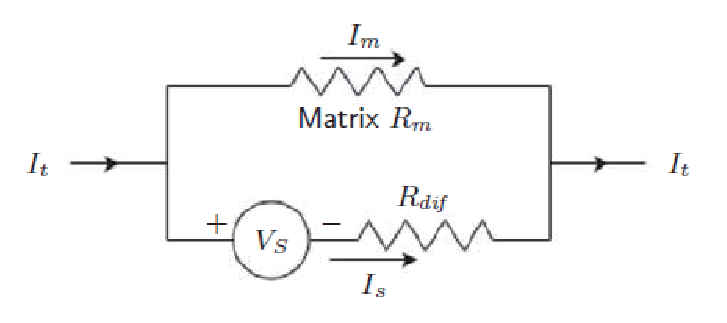
\includegraphics[scale=0.7]{chpt6/figs/fig6.11.eps}
	\caption{具有如6.25式$V_s$ vs. $I_s$特性的复合超导体的等效电路模型,旁路为基底点电阻$R_m$。
	超导体由理想电压源和差分电阻并联而成。}
\end{figure}

\subsubsection{问题6.3之解}
a) 根据$R_s$的定义,并使用6.25中的$V_s$,有:
\begin{align*}% page372 第1个 S3.1
R_s=\frac{V_s}{I_s}=\frac{V_c}{I_s}(\frac{I_s}{I_c})^2=\frac{V_c}{I_c}(\frac{I_s}{I_c})^{(n-1)} \tag{S3.1}
\end{align*}

代入$R_c=V_c/I_c$,S3.1成为:
\begin{align*}% page372 第2个 6.26a
R_s=R_c(\frac{I_s}{I_c})^{(n-1)} \tag{6.26a}
\end{align*}

$R_{dif}$表示超导体在$I_s$时的差分电阻,于是:
\begin{align*}% page372 第3个 S3.2
R_{dif}=\frac{\partial V_s}{\partial I_s}=\frac{nV_c}{I_c}(\frac{I_s}{I_c})^{(n-1)} \tag{S3.2}
\end{align*}
\begin{align*}% page372 第4个 6.26a
R_{dif}=nR_c(\frac{I_s}{I_c})^{(n-1)} \tag{6.26a}
\end{align*}

在S3.2中取偏微分是因为实际情况下$I_c$对温度的依赖必须在$I_s>I_c$区间的分析中予以考虑,该区间复合导体
会被加热,此处将被加热至77.3 K以上。

b) 电路必须满足下面的电流电压方程:
\begin{align*}% page372 第5个S3.3a
I_t=I_m+I_s \tag{S3.3a}
\end{align*}
\begin{align*}% page372 第6个S3.3b
V_m=R_mI_m=V_s=V_c(\frac{I_s}{I_c})^{n} \tag{S3.3b}
\end{align*}

作为例子,我们计算$I_t=90$ A时的$I_m$。从S3.3a,我们有$I_s=90\ \mathrm{A}-I_m$。
将之代入S3.3b,有:
\begin{align*}% page372 第6个S3.3c
3\times 10^{-4}\ \Omega\times I_m[\ \mathrm{A}]=10^{-5}V(\frac{90\ \mathrm{A}-I_m[\ \mathrm{A}]}{100\ \mathrm{A}})^{15} \tag{S3.3c}
\end{align*}

从S3.3c知,$I_m=$0.00686 A,故$I_s$=89.99314 A。

复合导体中的总热耗散功率$P_D$为:
\begin{align*}% page372 第7个S3.4
P_{cd}=R_mI_mI_t=V_sI_t \tag{S3.4}
\end{align*}

焦耳热耗散热流$g_{jcd}$简单的由$P_{cd}$除以复合导体的总冷却面积得到。

表6.5a给出了b)的解。


\begin{table}[htbp]\small
\centering
\caption{方程5.40在NbTi和YBCO材料的应用} 
\begin{tabular}{|c|c|c|c|c|c|c|}
\hline
 $I_t[A]$   &$I_m[A]$         &$I_s$[A]          &$R_mI_m[V]$
 &$P_{cd}[W]$      &  $g_{jcd}[W/cm^2]$    & $R_{dif}[\Omega]$      \\
 \hline
90  & 0.00686 & 89.99314 & 2.06$\times10^{-6}$ & 185$\times10^{-6}$  & 18.5$\times10^{-6}$ & 0.343$\times10^{-6}$ \\ \hline
100 & 0.0332  & 99.967   & 9.95$\times10^{-6}$ & 995$\times10^{-6}$  & 99.5$\times10^{-6}$ & 1.49$\times10^{-6}$  \\ \hline
120 & 0.483   & 119.517  & 145$\times10^{-6}$  & 17.4$\times10^{-3}$ & 1.74$\times10^{-3}$ & 18.2$\times10^{-6}$  \\ \hline
150 & 7.07    & 142.93   & 2.12$\times10^{-3}$ & 318$\times10^{-3}$  & 31.8$\times10^{-3}$ & 223 $\times10^{-6}$  \\ \hline
300 & 126.75  & 173.25   & 38.0$\times10^{-3}$ & 11.4 & 1.14 & 3.29$\times10^{-3}$  \\ \hline
500 & 315.88  & 184.12   & 94.8$\times10^{-3}$ & 47.4 & 4.74 & 7.72$\times10^{-3}$  \\ \hline
\end{tabular}
\end{table}


c) 即使复合导体被沸腾液氮很好的冷却,它的温度必然升高以将焦耳热传至制冷剂。
这里,液氮沸腾温度为77.3 K,随热流密度增加,导体温升在核态沸腾区域可高达$\sim 10$ K。
方程6.25a中最明显的温度依赖参数是$I_c$,它随温度增加而降低;LTS和HTS的$n$值对温度的依赖关系少见文献报道,
我们假定其为常数。在等效电路中,如果是纯金属基底,$R_m$在低温区可视为常数,但在温度超过$\sim 30$ K后
近似线性随温度增加。$I_c$可以认为随温度$T$线性降低。$(I_s/I_c)^n$项于是随温度(焦耳热)剧烈增加。
接下来,在问题6.4中,我们将做$I_c,R_m$为温度依赖的电路分析。

d) e)结果总结在表6.5b。

注意到,在$I_t>I_c=100$ A时,$n$值越小,$I_m, R_m I_m=V_s(I_s),P_{cd},g_{jcd},R_{dif}$也越小;
在$I_t<100$ A时,相反的结论成立。
这是很实际的问题。例如,在$I_t$=150 A时,对$n=15$的复合导体,$R_mI_m$=2.12 mV;
而$n=60$的复合导体这个值时11.3 mV:很明显,就检测电阻性电压而言,显然$n=60$的导体要比$n=15$的好。 

\begin{table}[htbp]\small
\centering
\caption{方程5.40在NbTi和YBCO材料的应用} %6.5b
\begin{tabular}{|c|c|c|c|c|c|c|}
\hline
  $I_t[A]$  &   $ I_m[A]$     &  $I_s[A]$        & $R_mI_m$      &
  $P_{cd}[W]$   &  $g_{jcd}[W/cm^2]$     & $R_{dif}[\Omega]$      \\
  \hline
\multicolumn{7}{|c|}{n=30}                              \\ \hline
90  & 0.00141 & 89.9986  & 0.424$\times10^{-6}$ & 38.1$\times10^{-6}$ &
3.81$\times10^{-6}$  & 0.127$\times10^{-6}$ \\ \hline
100 & 0.0330  & 99.967   & 9.90$\times10^{-6}$  & 990$\times10^{-6}$  &
99.0$\times10^{-6}$  & 2.97$\times10^{-6}$  \\ \hline
120 & 3.37    & 116.63   & 1.01$\times10^{-3}$  & 121$\times10^{-3}$  &
12.1$\times10^{-3}$  & 260$\times10^{-6}$   \\ \hline
150 & 25.27   & 124.73   & 7.58$\times10^{-3}$  & 1.14 &
114$\times10^{-3}$   & 1.82$\times10^{-3}$  \\ \hline
300 & 167.16  & 132.8    & 50.1$\times10^{-3}$  & 15.0 & 1.50  &
11.32$\times10^{-3}$ \\ \hline
500 & 363.67  & 163.33   & 109$\times10^{-3}$   & 54.6 & 5.46  &
24.0$\times10^{-3}$  \\ \hline
\multicolumn{7}{|c|}{n=60}                              \\ \hline
90  & 0.00006 & 89.99994 & 0.018$\times10^{-6}$ & 1.60$\times10^{-6}$ &
0.162$\times10^{-6}$ & 0.012$\times10^{-6}$ \\ \hline
100 & 0.0327  & 99.9673  & 9.81$\times10^{-6}$  & 981$\times10^{-6}$  &
98.1$\times10^{-6}$  & 5.89$\times10^{-6}$  \\ \hline
120 & 10.02   & 109.98   & 3.01$\times10^{-3}$  & 361$\times10^{-3}$  &
36.1$\times10^{-3}$  & 1.64$\times10^{-3}$  \\ \hline
150 & 37.57   & 112.43   & 11.3$\times10^{-3}$  & 1.69 &
169$\times10^{-3}$   & 6.02$\times10^{-3}$  \\ \hline
300 & 184.55  & 115.45   & 55.4$\times10^{-3}$ & 16.6 & 1.66  &
28.8$\times10^{-3}$  \\ \hline
500 & 383.14 & 116.86 & 114.9$\times10^{-3}$ & 57.5 & 5.75 &
59.0$\times10^{-3}$ \\ \hline
\end{tabular}
\end{table}


\subsection{问题6.4:电流脉冲下的YBCO}
此处,我们考虑一个10 mm宽的YBCO超导带样品,由77 K的沸腾液氮冷却。
图6.12a给出了导体截面的示意图。导体的一侧由G10带绝缘;另一侧在银层外焊了铜层,总的Cu/Ag层厚度为
55 $\mu$m;Cu表面与沸腾液氮接触。传输电流$I_t(t)$流过复合导体。
如图6.12b中的虚线所示,它从100 A开始,快速升高至300 A,保持0.31 s后回到100 A。
5 cm长的导体上的电压$V_{cd}(t)$如图6.12b中的实线所示。

尽管实际的HTS磁体非常可能绝热运行,但对于$V_s-I_s$关系图等的测量总是将测试样品置于冷却良好的恒温环境
为佳,对HTS,将之浸泡于液体工质中即可轻松实现。
\begin{figure}[htbp]
	\centering
	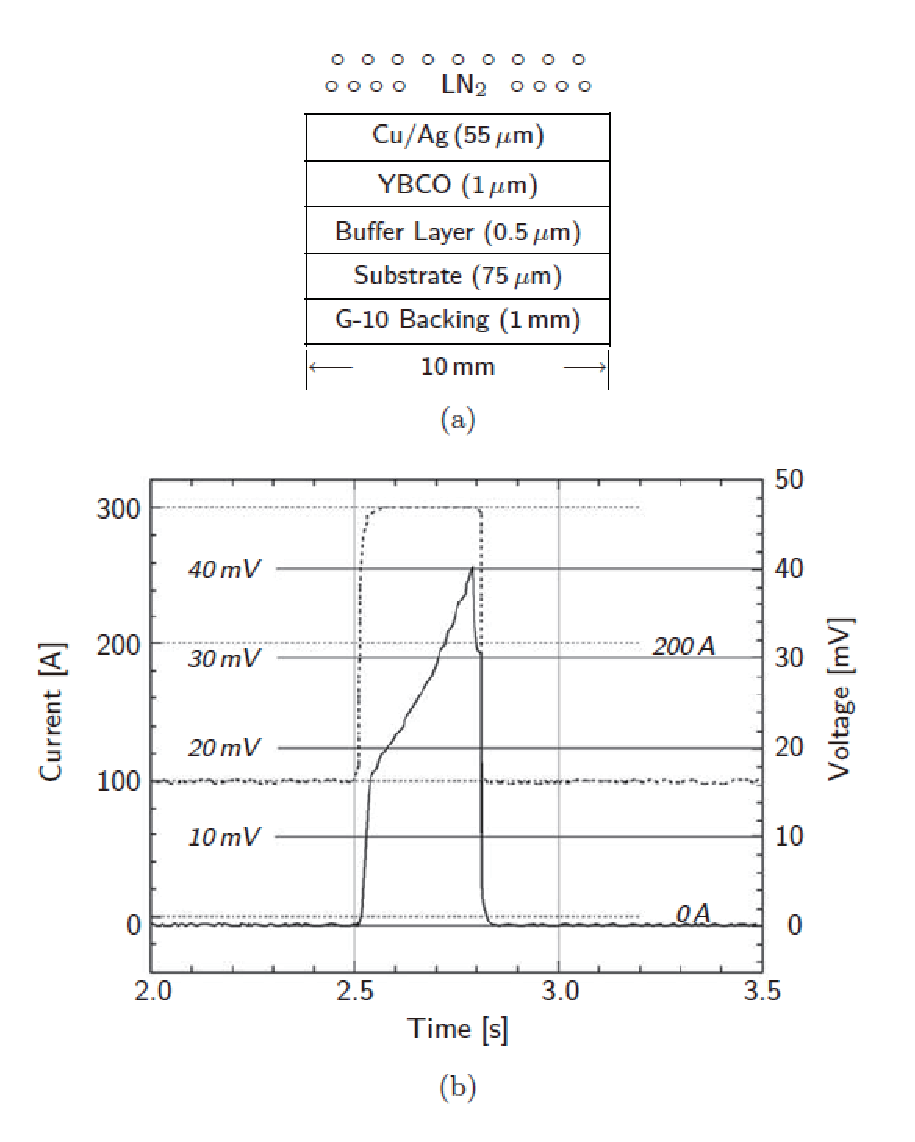
\includegraphics[scale=0.5]{chpt6/figs/fig6.12.eps}
	\caption{(a)10 mm宽的YBCO超导带样品截面图;Cu/Ag面暴露于沸腾液氮;(b)施加过流脉冲后记录的
		传输电流(虚线)和电压(实线)随时间变化的轨迹。}
\end{figure}

对这个YBCO带材,我们可以使用以下依赖于温度的正常金属基底:
\begin{subequations}
	\begin{align}
	R_m(T)&=0.190+1.530(\frac{T-77}{293-77})\ [\ \mathrm{m}\Omega]\\
	I_c(T)&=100(\frac{93-T}{93-77})[\ \mathrm{A}]\\
	V_s(T)&=5[\frac{I_s(T)}{I_c(T)}]^{10} [\ \mathrm{\mu V}]
	\end{align}
\end{subequations}

式中,$T$的单位是K。方程6.27a在77-293 K内有效;方程6.27b和6.27c仅在$\sim $77-93 K内有效。

a) 应用图6.12b,在电流脉冲的初始部分($t\simeq$2.54 s和$I_t$=290 A),此时假设导体仍然为77 K
是合理的,我们有:$V_{cd}(t=2.54)\simeq$18 mV。为了满足图6.11电路模型要求的电压电流关系,计算:
1) $I_s$;2)$I_m$;3) $V_{cd}$。

此处计算得到的$V_{cd}$等于测量值18 mV吗?

b) 在本实验测出的$V_{cd},I_s,n$中,最不准确的是$n$。证明,方程6.27c中代入$n=12.24$给出a)中的
$V_{cd}$=18 mV。

c) 在脉冲期间,$V_{cd}(t)$持续增加,达到峰值40 mV---在脉冲结束前$V_{cd}(t)$的跌落应该是由冷却的突然
改善造成的。计算当$V_{cd}(t=2.79)=40$ mV时复合导体表面的热流密度$p_{cd}$。

d) 假设Cu-Ag和YBCO层温度相同,计算$V_{cd}(t=2.79)=40$ mV时的温度。$n$取12.24。


\subsubsection{问题6.4之解}
a) 电路必须同时满足电流和电压要求:
\begin{align*}% page376 第1个S4.1a
I_t=I_s+I_m \tag{S4.1a}
\end{align*}
\begin{align*}% page376 第2个S4.1b
R_mI_m=V_s(I_s) \tag{S4.1b}
\end{align*}

代入合适的值,有:
\begin{align*}% page376 第3个S4.2a
I_s=(290\ \mathrm{A})-I_m \tag{S4.2a}
\end{align*}
\begin{align*}% page376 第4个S4.2b
(0.19\times10^{-3}\ \Omega)I_m=(5\times10^{-6}\ \mathrm{V})(\frac{290\ \mathrm {A}-I_m}{100\ \mathrm{A}})^{10} \tag{S4.2b}
\end{align*}

由方程S4.2b解$I_m$,我们有:1) $I_m$=70 A。一旦$I_m$已知,$I_s$和$V_{cd}$则容易计算:
2) $I_s$=220 A; 3)$V_{cd}$=13.3 mV。也即,计算值与测量值18 mV并没有很好的吻合。

b) 在77 K,我们知道$R_m=0.19\ \mathrm{m}\Omega$。所以,使用$R_m I_m$=18 mV解出$I_m$,我们有:
$I_m$=94.74 A;因此。$I_s$=290 A-94.74 A=195.26 A。将这些值代入6.2c,并将10用未知的$n$代替,有:
\begin{align*}% page376 第5个S4.3
(18\times10^{-3}\ \mathrm{V})=(5\times10^{-6}\ \mathrm{V})(\frac{195.26\ \mathrm{A}}{100\ \mathrm{A}})^n \tag{S4.3}
\end{align*}

解出$n$,有$n$=12.24。计算值和测量值之间的明显的$\sim 20\%$的误差是正常的,因为$n$是从$V_s$ vs. $I_s$
测量值中导出的。不过,由于$n$是指数,它很小的误差会给其他参数带来很大的误差。

c) 这段5 cm长复合导体的总耗散功率$P_{cd}$为$P_{cd}=V_{cd}I_t$。
因此,$P_{cd}=$40 mV$\times$300 A=12 W。
因为接触制液氮的总基底面积是5 $\mathrm{cm^2}$(边缘面积忽略),
我们有热流密度$p_{cd}=2.4\ \mathrm{W/cm^2}$。
该值小于液氮核态沸腾的峰值热流密度$\sim 10\ \mathrm{W/cm^2}$。

d) 电路要求与a)相同,除了温度不再是77 K。仅已知参数为$V_{cd}=$40 mV。这样,对基底由:
\begin{align*}% page376 第6个S4.4
V_{cd}=40\times10^{-3}\ \mathrm{V}=R_m(T)I_m ]\tag{S4.4}
\end{align*}

联立S4.4和6.27a,有:
\begin{align*}% page376 第7个S4.5a
10\times10^{-3}=[{[0.190+1.530(\frac{T-77}{293-77})]^\times10^{-3}\ \Omega}]I_m(T) \tag{S4.5a}
\end{align*}
\begin{align*}% page376 第8个S4 .5b 
I_m(T)=\frac{40\times10^{-3}\ \mathrm{V}}{[0.190+1.530(\frac{T-77}{293-77})]\times10^{-3}\ \Omega}I_m(T) \tag{S4.5b}
\end{align*}
\begin{align*}% page376 第9个S4 .5c
=\frac{40}{0.190+1.530(\frac{T-77}{293-77})}\ \mathrm{A} \tag{S4.5c}
\end{align*}

超导侧有同样的$V_{cd}$,于是:
\begin{align*}% page377 第1个S4.6
40\times10^{-3}\ \mathrm{V}=(5\times10^{-6}V)[\frac{300A-I_m(T)}{I_c(T)}]^{12.24} \tag{S4.6}
\end{align*}

由方程S4.5c和6.27b分别给出的$I_m(T)$和$I_c(T)$,我们有:
\begin{align*}% page377 第2个S4.7
40\times10^{-3}\ \mathrm{V}=(5\times10^{-6}V)[\frac{300\ \mathrm{A}-\frac{40\ \mathrm{A}}{[0.190+1.530(\frac{T-77}{293-77})]}}{(100\ \mathrm{A})(\frac{93-T}{93-77})}]^{12.24}\tag{S4.7}
\end{align*}

方程S4.7可以化简为:
\begin{align*}% page377 第3个S4.8
8000=[\frac{16(406200T-28027799)}{(93-T)(135400T-6793895)}]^{12.24} \tag{S4.8}
\end{align*}

解出$T$,有$T$=83.125 K。这等价于超导体表面和77.3 K沸腾液氮之间约6 K的温差;
对液氮来说,这个温差肯定是位于核态沸腾区域的。图6.13给出了液氮沸点为77.3 K的热流数据。对应6.4的数据点
在图中以实心圆点标出。
\begin{figure}[htbp]
	\centering
	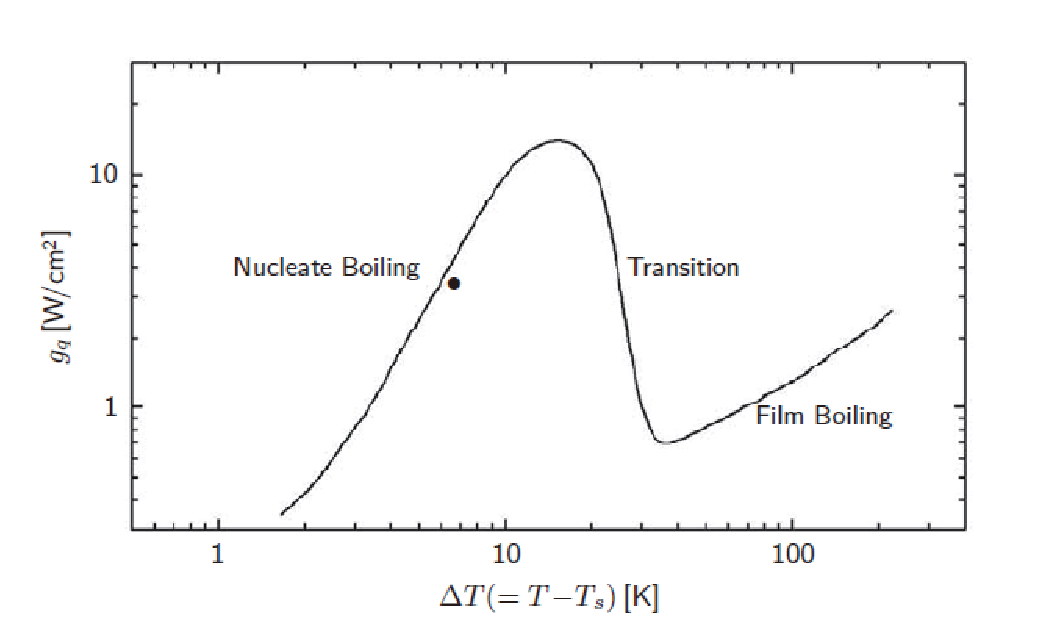
\includegraphics[scale=0.6]{chpt6/figs/fig6.13.eps}
	\caption{沸点为77.3 K的液氮的典型热流密度数据。对应c)和d)的数据点在图中以实心点标出。}
\end{figure}

\subsection{讨论6.6:CIC导体}
在考虑稳定性和寻找浸泡冷却替代方案的时候,Hoenig和Montgomery在1970年代初提出了CIC(cable-in-conduit,
沟槽电缆)导体的概念[6.21]。
实际上,寻找以迫冷方式取代浸泡方式冷却超导磁体的思路在1960年代中期就由Morpurgo提出了[6.22],他提出了
一种类似阻性磁体的水冷铜线的带冷却孔的超导体。
在传热方面,CIC导体要优于单孔导体,这是因为在相同的制冷剂截面下,电缆提供了比单孔导线内壁面更大的冷却面积。
基于这个思想,实现了一种将超导股线置于防漏沟槽中,其中通入超临界氦的实例,这种构造使得制冷剂几乎完全渗透
到了所有绕组。图6.14给出了CICC的示意图。基于这种基础概念,现在已有多个变种。

在CICC开始发展滞后,它的第二个有利特征(最初忽略了)才被认识到:内秉的加强。
大型(绕组内径大于1 m)和高场(大于10 T)的磁体几乎毫不例外的使用CIC导体。
大型、高场磁体通常是昂贵的。并且,它经常还是仅作为一个更大更昂贵设备比如聚变反应堆的部件而已;
磁体必须绝对稳定。
因为一个稳定的磁体必须保证绕组的所有部分的导体都得到良好的冷却,CIC导体因其特有的配置,自然的同时满足了
稳定性和强度的要求。

\textbf{A. 功率密度方程}

复合导体的基本功率密度方程除了冷却项更为明确外,和方程6.1相同:
\begin{equation}% page378 第1个6.28a
C_{cd}(T)\frac{\partial T}{\partial t}=\nabla.[k_{cd}(T)\nabla T]+\rho_{cd}(T)J_{cd_o}^2(t)+g_d(t)-(\frac{f_pP_D}{A_{cd}})h_{he}(T-T_{he})
\end{equation}

式中,$h_{he}$和$T_{he}$分别是传热系数和通过沟槽的迫流氦的温度。
当前所有CIC导体都是基于LTS的,由氦冷却。所以,上式中使用了$h_{he}$和$T_{he}$。
$T_{he}$的功率密度方程为:
\begin{align*}% page378 第2个6.28b
C_{he}(T_{he})\frac{\partial T_{he}}{\partial t}=(\frac{f_{p}P_D}{A_cd})h_{he}(T-T_{he})
\end{align*}

\begin{figure}[htbp]
	\centering
	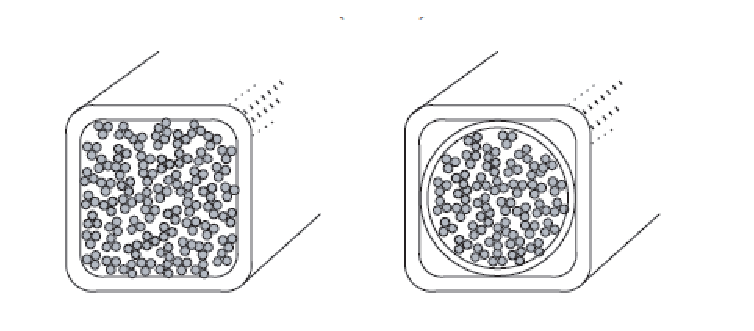
\includegraphics[scale=0.7]{chpt6/figs/fig6.14.eps}
	\caption{CIC导体实例。}
\end{figure}

\textbf{B. CIC导体的组成}

从图6.14可以得到,CIC导体包括:1) 电缆;2) 氦;3) 沟槽。下面简要描述三部分。

\textbf{电缆}

电缆一般是由多股组成的,每一股直径约1 mm或更小,各包含10-100$\mu$m直径的
NbTi或$\mathrm{Nb_3Sn}$超导体细丝;通常与超导细丝同等直径的铜丝会用于取代部分超导细丝组成股,
用以增强基底金属的截面积和/或减少电缆费用。
通常,3到7股被``绑扎"为所谓的``基本缆"。图6.14中可以看到基本缆是由三股构成的。
典型的CIC导体的截面至少为1或2 cm截面---聚变磁体的可能超过5 cm---因此,运行电流可以很大,$I_{op}$
至少10 kA,部分聚变磁体的可接近100 kA。
为了实现这个高$I_{op}$要求,比如(典型的)3/5/7组基本缆进一步绑扎形成所谓``二级缆",
如此继续直到满足要求。

表6.6列出了三种CIC导体:45 T NHMFL混合磁体的线圈A和C;ITER环形场线圈设计的一种建议CIC导体。
45 T混合磁体在运行,ITER线圈尚处于设计阶段,尽管已有多种不同模型版本在运行。
表6.6的第一部分列出了这些线圈所用电缆的参数。

\textbf{氦}

超临界态(压力超过其临界压力227.5 kPa或2.25atm)的氦以迫冷方式通过额定运行压力$P_{op}\sim$3-5 atm绕组。
运行温度$T_{op}$通常由氦维持在其临界温度5.2 K之下,循环氦进入绕组前典型温度为4.3-4.5 K。
45 T混合磁体中,氦被过冷到超流态,额定运行温度为1.8 K,额定运行温度为1 atm。
超流氦的独特性质(高热导率、低粘度)让这个系统可以简单地依赖``自然对流"而不是迫流
来将热耗散输运到绕组外部的热交换器。三个线圈的氦参数在表6.6的中部。

对迫流氦,其换热系数$h_{he}[\mathrm{W/cm^2 K}]$是基于所谓的Dittus-Boelter-Giarratano-Yaskin
关系[6.23]的:
\begin{equation}% page379 第1个6.29
h_{he}=0.0259(\frac{k_{he}}{D_{hy}})Re^{0.8}Pr^{0.4}(\frac{T_{he}}{T_{cd}})^{-0.716}
\end{equation}

式中,$k_{he}$、Re、Pr分别是氦的热导率、雷诺数和普朗特数;$D_{hy}$是水力直径;
$T_{cd}$是导体温度。3.5 atm和4.5 K下对应Re=$10^4$和Re=$10^5$的传热热流$g_q$值如图6.3。

\begin{table}[htbp]\small
\centering
\caption{方程5.40在NbTi和YBCO材料的应用} %6.6
\begin{tabular}{|l|c|c|c|}
\hline
\multicolumn{1}{|c|}{CIC Conductor Coil}
& \multicolumn{2}{c|}{45-T Hybrid Magent}
& \multirow{2}{*}{\begin{tabular}[c]{@{}c@{}}ITER\\ TF
Coil\end{tabular}} \\ \cline{1-3}
Parameters
& Coil A
& Coil C
&
\\ \hline
Nominal $I_{op} $[kA]
& \multicolumn{2}{c|}{10}
& 50
\\ \hline
\hline
Total area (A$_{cic}$){[}mm$^2${]} & 209.94 & 196.29 & 2601 \\ \hline
\begin{tabular}[c]{@{}l@{}}Basic Cable$\sharp$starands\\ Strand
diameter,$D_{st}$ {[}mm{]}\\ Cable Patterns\\ Total strand
number,Nst\\ Conductor area ,$A_{cd}$ {[}mm$^2${]}\\
$A_{sc}$+$A_{\overline{m}}$ {[}mm$^2${]}\\$ A_m$
{[}mm$^2${]}\\ $A_cd$/$A_{cic}$\end{tabular} &
\begin{tabular}[c]{@{}c@{}}6 Nb$_3$Sn/Cu+1Cu\\ 0.433\\
7$\times3\times5\times5$\\ 525\\ $79.44^\ast$\\ 25.19\\ 54.25\\
0.38\end{tabular} & \begin{tabular}[c]{@{}c@{}}3 NbTi/Cu\\ 0.810\\
3$\times3\times3\times5$\\ 135\\ $70.49^\ast$\\ 11.25\\ 59.14\\
0.36\end{tabular} & \begin{tabular}[c]{@{}c@{}}6 Nb$_3$Sn/Cu\\ 0.810\\
3$\times(4^3)\times6$\\ 1152\\ 593.6\\ 94.74\\ 498.05\\
0.23\end{tabular} \\ \hline
\begin{tabular}[c]{@{}l@{}}Helium\\ Nominal P$_{op }$ {[}atm{]}\\
Nominal
T$_{op }$ {[}K{]}\\ Nominal fiow rate {[}g/s{]}\end{tabular}
& \multicolumn{2}{c|}{\begin{tabular}[c]{@{}c@{}}Superfluid$\dagger$\\
1\\ 1.8\\
not-forced;natural convection\end{tabular}}
& \begin{tabular}[c]{@{}c@{}}Supercritical\\ 5\\ 4.5\\ 10\end{tabular}
\\ \hline
\begin{tabular}[c]{@{}l@{}}$D_{hy}\ddagger $ {[}mm{]}\\ Flow
area$\dagger\dagger(A_q)$
{[}mm$^2${]}\\ $A_q/A_{cic}$\end{tabular}
& \begin{tabular}[c]{@{}c@{}}227.3\\ 50.30\\ 0.24\end{tabular}
& \begin{tabular}[c]{@{}c@{}}109.4\\ 36.50\\ 0.19\end{tabular}
& \begin{tabular}[c]{@{}c@{}}933.1\\ 276\\ 0.106\end{tabular}
\\ \hline
\multirow{2}{*}{\begin{tabular}[c]{@{}l@{}}Conduit Material\\
Area($A_S$)
{[}mm$^2${]}\\ height$\times$width {[}mm$\times$mm{]}\\ wall
thickness {[}mm{]}\\
outer corner radius {[}mm{]}\\ A$_S/A_{cic}$\end{tabular}}
& \multicolumn{2}{c|}{Stainless steel$\ddagger\ddagger$}
& \multirow{2}{*}{\begin{tabular}[c]{@{}c@{}}Incoloy\\ 1466.9\\
51$\times51$\\
2.86\\ \\ 0.56\end{tabular}} \\ \cline{2-3}
 &
 \begin{tabular}[c]{@{}c@{}}80.20\\
 16.22$\times13.71$\\
 1.64\\
 3.40\\
 0.38\end{tabular}
 &
 \begin{tabular}[c]{@{}c@{}}89.30\\
 15.85$\times$13.74\\
 2.00\\
 4.77\\
 0.45\end{tabular}
 &
 \\
 \hline
\end{tabular}
\end{table}


\textbf{沟槽}

沟槽装入捆扎后的电缆股,提供制冷剂空间。制冷剂通常是迫流超临界氦,但如果是超流氦也可以不迫流,
就如45 T混合磁体的线圈那样。
$\mathrm{Nb_3Sn}$细丝是脆的,应变不能超过$\sim 0.3\%$,$\mathrm{Nb_3Sn}$反应的最后的热处理
必须在未反应股装入沟槽后并绕成线圈后进行。
在1980年代,一种镍铁基合金Incoloy 908被优选用为沟槽金属,但近来多数沟槽都使用316 LN不锈钢了---
LN表示低碳高氮。

\textbf{C. 稳定性}

从1970年代初开始,CIC导体的稳定性就引起了很大的注意。
早期的一个重要结论就是在1977年观察到了CIC导体及时在没有工质净流入的情况下也能``失超恢复``[6.24]。
很明显,受热区域的热致高速局部制冷剂流动提供了失超恢复的必要冷量。

CIC导体稳定性工作一个早期重要里程碑是Lue、Miller和Dresner在1979年发现了存在于特定运行工况
下可能存在多值稳定裕度[6.25]。
这里,能量裕度$\Delta e_h$定义为最大耗散能量密度脉冲(单位股体积)与导体载有戈丁传输电流仍能保持
超导态的最大电流之比。图6.15给出了恒定运行温度、磁场、工质流量下的典型
$\Delta e_h$ vs. $I_t/I_{c_o}$。
这里,$I_t$是传输电流,$I_{c_o}(T_{op},B_0)$是临界电流。
具有多值稳定裕度的``双重稳定性"区域发生于$I_t、I_{c_o}\sim 0.5$附近。
小于该区域的部分称为良好冷却区,大于部分称为不良冷却区[6.26]。

为了确保满足大型超导磁体如聚变磁体的稳定运行要求,ITER磁体设计运行于良好冷却区域,即$I_t$小于
$I_{lim}$:
\begin{align}% page381 第1个6.30
I_{lim}=\sqrt{\frac{A_mf_p\ \mathrm{P}_Dh_{he}(T_c-T_{op})}{\rho_m}}
\end{align}

注意到,$I_{lim}$满足Stekly判据,即方程6.19中,有$I_{lim}=I_{c_o},\alpha_{sk}=1$。
\begin{figure}[htbp]
	\centering
	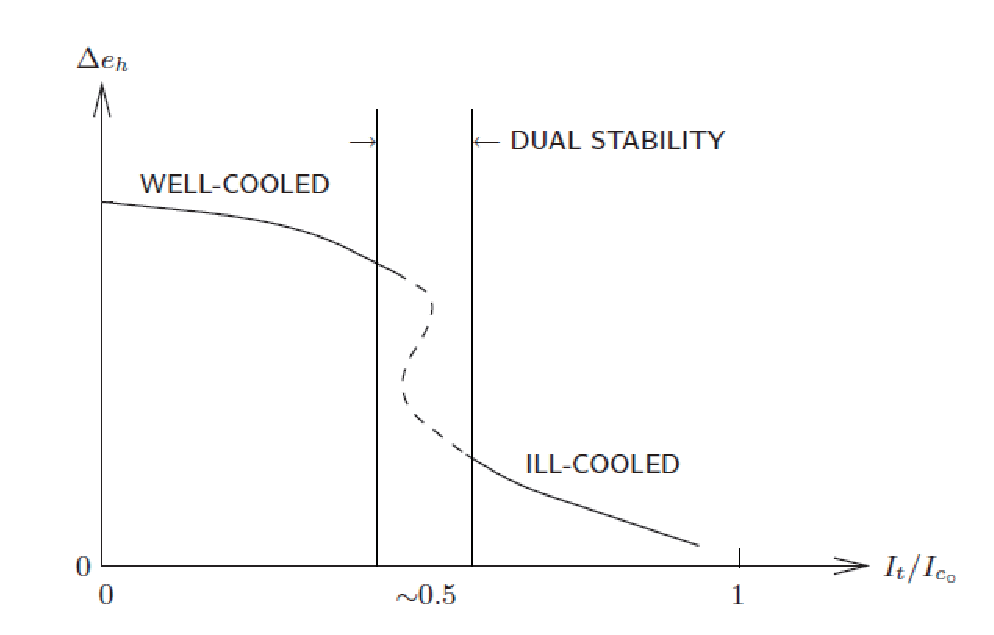
\includegraphics[scale=0.7]{chpt6/figs/fig6.15.eps}
	\caption{CIC导体的一般能量裕度 vs. 归一化传输电流关系。}
\end{figure}

\textbf{D. 其他事项}

\textbf{交流损耗}

因为聚变超导磁体处于时变磁场中,在CIC导体内部将发生交流损耗。如果处理交流损耗是CIC导体设计的一个
主要课题[6.27-6.50]。交流损耗将在第七章讨论。

\textbf{接头}

CIC导体要同时处理载流的股和载工质的沟槽。所以,CIC导体的连接相比于在沟槽能连接两个无约束导体更为困难。
为了处理这个问题,已经发展了多种技术[6.51-6.57]。

\textbf{升流速率极限}

由成缆股丝构成的CIC导体有时候会遇到一种称为``升流速率极限"的现象,该现象是一种不稳定性,会令导体在其
设计运行电流下失超。这个不稳定现象仅在导体升流速率超过临界速率或置于快速变化的背景场中载有恒定电流的导体
内出现。很明显,沟槽内缆丝的非均流主要是源于其电感和电阻不等。在过去的十多年,该问题
已得到较为深入的研究[6.58-6.62]。
升流速率极限不会在运行电流$I_{lim}$之下的电缆中发生---这或许是大型磁体运行于由$I_{lim}$限定的保守电流
下的另一个原因。

\subsection{问题6.5:冷却复合物导体的伏安关系}
本问题考察浸泡于4.2 K液氦中的复合超导体的V-I特性;
我们将在三种不同冷却条件下考虑V-I特性。
超导体参数如下:$T_{op}$=4.2 K下的临界电流$I_{c_o}$=1000 A;基底金属电阻率$\rho_m=4\times 10^{-10}\ 
\Omega m$;基底总截面积$A_m=2\times 10^{-5}\ \mathrm{m^2}$;
总导体周长$P_{cd}=2\times 10^{-2}$ m,暴露于液氦部分:$f_p P{cd}$;
传热系数$h_q=10^4\ \mathrm{W/m^2K}$。
$V$的带材测试长度为$\ell=0.1$ m。为了推到V-I关系,假定$I_c(T)$按方程6.12给出。

a) 在$I<I_{c_o}$,我们有$V$=0 V。$I\ge I_{c_o}$,证明$V$可由下式给出:
\begin{equation}% page383 第1个6.31
V=\frac{R_m(I-I_{co})}{1-\frac{R_mII_{co}}{f_pP_{cd}\ell h_q(T_c-T_{op})}}
\end{equation}

式中,$R_m=\rho_m \ell/A_m$。假设导体出于热平衡态,即$T_{op}+\Delta T$的导体的阻性热耗散被冷量平衡。
注意到$I_m=I-I_s$,其中$I_m$是基底电流,$I_s$是超导体在$T=T_{op}+\Delta T$时的电流,如方程6.12所给。

b) 通过定义两个无量纲参数$v\equiv V/R_m I_{c_o}, i\equiv I/I_{c_o}$,加上Stekly参数$\alpha_{sk}$
(方程6.19),证明无量纲电压可由下式给出:
\begin{equation}% page383 第2个6.32
\ \mathrm{u}(\ \mathrm{i})=\frac{\ \mathrm{i}-1}{1-\alpha_{ski}}
\end{equation}

c) \textbf{工况1:}$f_p=1(\alpha_{sk}=0.1)$。在$T_c$=5.2 K($T_{op}$=4.2 K)时,计算$i=1,1.1,1.5,1.2$
时的$v$。

d) \textbf{工况2:}$f_p=0.1(\alpha_{sk}=1)$。证明在$i=1$时,不能确定$v$。

e)\textbf{工况3:}$f_p=0.05(\alpha_{sk}=2)$。这里,表面积近乎与液氦热绝缘,导体将不稳定。Stekly
在他的实验中使用实际电源观察到,电源电流在回到初始电流和相应的电压($v=i$线)前,
突然从设计值跌落,与正的负载电压匹配[6.63]。
由6.31导出的6.32基于$i<1$时$v=0$这一前提,在$i>1$稳态工况下不成立。你可以使用这个方程找到当$i$=1,0.9,0.8,0.75和0.707时的$v$值。

f) 画出上文研究的三种工况下的$v(i)$图。用实线画出$v=i$。在三种工况上分别标上对应$\alpha_{sk}$值。


\subsubsection{问题6.5之解}
a) 在$I> I_{c_o}$时,电势$V$由$R_m(I-I_s)$给出,其中$I_s$是超导体电流,即$I_s=I_c(T)$。
焦耳热$G_j(T_{op}+\Delta T)$于是为:
\begin{align*}% page384 第1个S5.1
G_{j}(T_{op}+\triangle T)&=VI=R_m\{I-I_{co}[\frac{T_c-(T_{op}+\Delta T)}{T_c-T_{op}}]\}I\\
&=R_mI[(I-I_{co})+\frac{I_{co}\Delta T}{T_c-T_{op}}] \tag{S5.1}
\end{align*}

$G_j(T_{op}+\Delta T)$由冷量匹配,冷量由$f_pP_{cd}\ell h_q(T_c-T_{op})=f_pP_{cd}\ell h_q\Delta T$给出。
令两个功率相等,解出$\Delta T$,有:
\begin{align*}% page384 第2个S52
\Delta T=\frac{R_mI(I-I_{c_o})(T-T_{op})}{f_pP_{cd}\ell h_q(T_c-T_{op})-R_mI_{c_o}I} \tag{S5.2}
\end{align*}

联立S5.1和S5.2,解出$V$:
\begin{align*}% page384 第3个S5.3a
V=R_m\{(I-I_{c_o})+\frac{I_{c_o}}{T_c-T_{op}}[\frac{R_mI(I-I_{co})(T_c-T_{op})}{f_pP_{cd}\ell h_q(T_c-T_{op})-R_mI_{c_o}I}]\} \tag{S5.3a}
\end{align*}
\begin{align*}% page384 第4个S5.3b
=R_m(I-I_{c_o})+\frac{R_m^2I_{c_o}(I-I_(co))}{f_pP_{cd}\ell h_q(T_c-T_{op})-R_mI_{c_o}I} \tag{S5.3b}
\end{align*}

由S5.3b,我们有:
\begin{align*}% page384 第5个6.31
V=\frac{R_m(I-I_{co})}{1-\frac{R_mII_{co}}{f_pP_{cd}\ell h_q(T_c-T_{op})}} \tag{6.31}
\end{align*}

b) 在$\alpha_{sk}$中,用$R_m/\ell$替代$\rho_m/A_m$,我们重写方程6.31:
\begin{align*}% page384 第6个
V=\frac{R_m(I-I_{co})}{1-\alpha_{sk}(I/I_{co})} \tag{S5.4}
\end{align*}

从中,可以得到:
\begin{align*}% page384 第7个
v(i)=\frac{i-1}{1-\alpha_{sk}i} \tag{6.32}
\end{align*}

c) $R_m=\rho_m \ell/A_m=2\times 10^{-6}\ \Omega$。代入$f_p=1$,有:
\begin{align*}% page384 第8个
\alpha_{sk}&=\frac{\rho_mI_{co^2}}{f_pP_{cd}A_mh_q(T_c-T_{op})}\\
&=\frac{(4\times10^{-10}\ \Omega\mathrm{m})(100\ \mathrm{A})^2}{(1)(2\times10^{-2}\ \mathrm{m^2})(10^4\ \mathrm{W/m^2K})(5.2\ \mathrm{K}-4.2\ \mathrm{K})}=0.1
\end{align*}

于是,方程6.32表示为:
\begin{align*}% page384 第10个
v(i)=\frac{10(i-1)}{10-i} \tag{S5.5}
\end{align*}

部分$i$值下的$v(i)$值如表6.7所列。

\begin{table}[htbp]\small
\centering
\caption{方程5.40在NbTi和YBCO材料的应用} %6.8
\begin{tabular}{|c|c|c|c|c|}
\hline
i & 1 & 1.1  & 1.5  & 2    \\ \hline
u & 0 & 0.11 & 0.59 & 1.25 \\ \hline
\end{tabular}
\end{table}


\begin{table}[htbp]\small
\centering
\caption{方程5.40在NbTi和YBCO材料的应用} %6.8
\begin{tabular}{|c|c|c|c|c|c|c|c|}
\hline
i & 1 & 0.9   & 0.8   & 0.75 & 0.725 & 0.707 & $\leq$0.707 \\ \hline
u & 0 & 0.125 & 0.333 & 0.5  & 0.611 & 0.707 & 0     \\ \hline
\end{tabular}
\end{table}


d) 当$f_p=0.1$时,$\alpha_{sk}$变为1。对$i<1$,根据定义,$v=0$。对$v>1$,由方程6.32,$v(i)=i$。
在$i=1$时,$v(i)$不能确定;物理上,如讨论6.1所指出的,这意味着$v$可以是$i=1$竖线上的任意点。
在$i=1(I=I_{c_o})$时,根据方程6.31,$V=0$。

e) 这里,$f_p = 0.05,\alpha_{sk} = 2$,我们可使用方程6.32计算$v(i)$。
如前所述,Stekly观察到[6.63]$v(i)$在$i=0.707$(这里计算的)和$i= 1$之间的双值,即$i$从0增长到1,$v=0$,
在$i=1$点,$v$突然出现,迫使$i$跌落(因为电源在电流$i=0$到$i=1$之间,电压很小,不能维持$i=1$的电流)。
首先,图6.16中,在$i=1--0.707$之间标记了$\alpha_{sk}=2$的$v$迹线称为$\alpha_{sk}$下的``恢复"(归一)电流。
然后,随着$i$减小到0.707之下,$v$回到0。 

f) 如图6.16。
\begin{figure}[htbp]
	\centering
	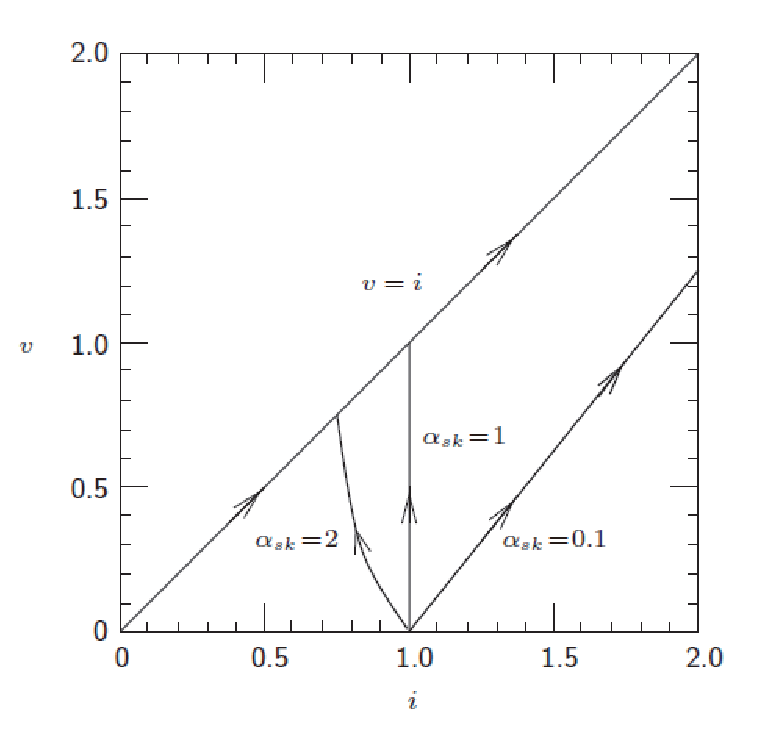
\includegraphics[scale=0.7]{chpt6/figs/fig6.16.eps}
	\caption{$\alpha_{sk}=0.1,1,2$下的归一化电压vs. 归一化电流迹线。}
\end{figure}


\subsection{问题6.6:混合III SCM的稳定性分析}
本问题处理混合III NbTi线圈的低温稳定性,它的导体特性见问题5.1的表5.1(混合III中的NbTi线圈
实际上使用了两种级别的NbTi导体;这里,简化为同一种级别的。)

NbTi线圈由32个双饼线圈组成,总绕组高度640 mm。
各饼的内径为658 mm,外径907 mm。图6.17给出了绕组的重要细节。
双饼线圈中的两个饼用0.5 mm厚浸渍环氧的薄绝缘层隔开。
相邻的双饼之间有1 mm厚的径向的绝缘垫片。
绝缘垫片平均占据了暴露于液氦中表面积的60\%。每一个双饼组中,氦仅浸润上饼上表面和下饼下表面。
因为液氦在1.8 K出现超流,不会出现气泡影响下饼的冷却。

\begin{figure}[htbp]
	\centering
	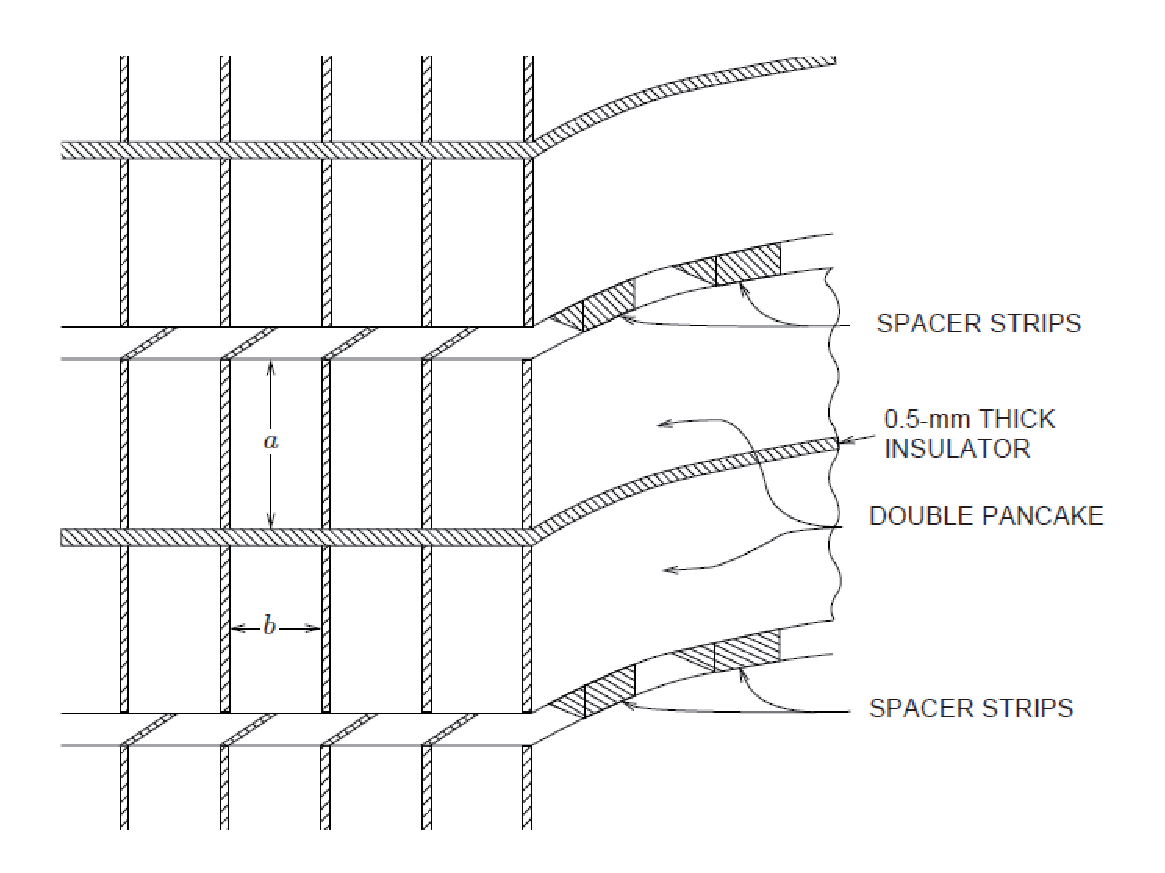
\includegraphics[scale=0.6]{chpt6/figs/fig6.17.eps}
	\caption{Winding details for the NbTi pancakes..}
\end{figure}

NbTi线圈(和$\mathrm{Nb_3 Sn}$线圈)设计为浸泡于1 atm和过冷1.8 K的超流液氦池中。
假设冷却主要是Kapitza热阻。所以,方程4.7给出的$q_k$应用于描写冷却:
\begin{align*}% page387 第1个
q_k=a_k(T^{n_k}_{cd}-T^{n_k}_b) \tag{4.7}
\end{align*}

式中,$T_{ck}$是导体温度(实际是导体表面的温度,也即金属基底的问题),$T_b$是液氦池温度。
可以取$a_k$=0.02 $\mathrm{W/cm^2 K^4}$,$n_k$=4.0(表4.7)。
在运行温度$T_{op}=1.8$ K($T_{op}=T_b$)时,线圈载有传输电流$I_{op}=2100$ A,暴露于最大外磁场$\sim$ 10 T下。
表5.1给出了有用的数据。

a) 为这个导体作一个合适的$I_c(T)$图,磁场为10 T,温区涵盖额定运行温度1.8 K到临界温度4.1 K。
从图中确定,传输电流$I_t$=2100 A下的电流分享温度$T_{cs}$,在图中标出。

b) 磁场10 T,温度$T_{op}=T_b$=1.8 K,$I_{op}$=2100 A,画并标出冷却和产热的功率密度和温度关系图。
根据图,阐述饼式线圈是否稳定,如果稳定,是基于何种判据?如果不稳定,解释原因。
为了回答这个问题,可以假定:1) 上面给出的$q(T)$在问题涉及的全温区都是合理的;2) 各饼内产生的热量可
通过1 mm径向通道自由传出。

c) FBNML之前建造的混合磁体的饼式线圈中,每一匝都由薄(0.4 mm)间隔片隔离,以使绕组通透,从而低温稳定。
在混合III项目的早期阶段,我们认真的考虑了匝间冷却隔离垫片的设计,但最终采用了无隔离片的方案。
结社混合III饼存在匝间隔离通道,在另一个图中简要画出功率密度和温度的关系图,
假定50\%的总导体周长直接暴露于液氦中,其他条件相同。同样,根据图,讨论饼线圈的稳定性。


\subsubsection{问题6.6之解}
a) 图6.18给出了这个导体的$I_c(T)$图,该图通过连接两个点而成:一点为1.8 K和10 T下的6000 A(表5.1),
另一点为4.7 K和10 T下的0 A(表5.1和图6.18)。电流分享温度由2100 A=$I_c(T_{cs})$给出,它是3.7 K的值。
\begin{figure}[htbp]
	\centering
	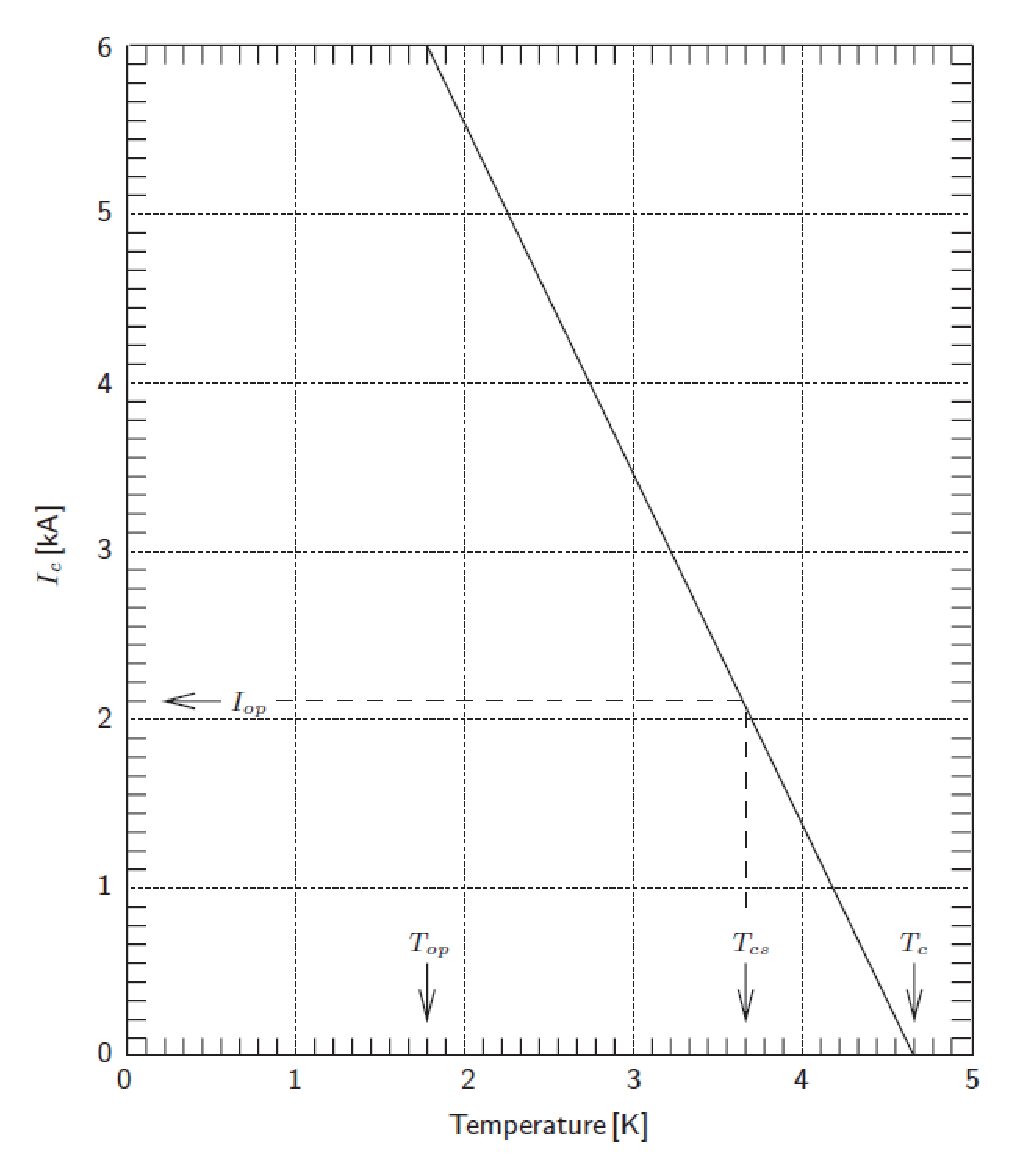
\includegraphics[scale=0.7]{chpt6/figs/fig6.18.eps}
	\caption{10 T混合III导体的$I_c$ vs. $T$图(实线)。$I_t$=2100 A是虚线,与实线交点对应$T_{cs}$=3.7 K}
\end{figure}

b) 首先计算$T\ge T_c$=4.7 K下有效的正常态下的$\hat{g}_j$。
和$g_j(T_c)=\rho_m I_{op}^2/A_m A_{cd}$不同,$\hat{g}_j$是正常态的产热通量密度(暴露于液氦中的导体单位表面积)。
也即,$\hat{g}_j=(A_{cd}/f_pP_{cd})g_j(T)$,其中$f_p P_{cd}$是暴露于液氦中的导体周长。
$A_{cd}$和$A_{m}$分别是全部导体和基底金属的截面积。
我么有:$A_{cd}=ab$,其中$a,b$分别是全部导体的宽和厚;$A_{m}=ab\gamma_{c/s}/(\gamma_{c/s}+1)$,
其中,$\gamma_{c/s}$是铜-超导体比率。于是我们有:$\hat{g}_j(T_c)=\rho_m I_{op}^2(\gamma_{c/s}+1)/\gamma_{c/s}abf_p P_{cd}$。

代入$I_t$ =2100 A,$\rho_m =4.5\times 10^{-10}\ \Omega \mathrm{m}$,$a$=9.2$\times 10^{-3}$ m, $b=2.6\times 10^{-3}$ m,$\gamma_{c/s}=3$,$f_p P_{cd}$ =(0.4)(2.6$\times 10^{−3}$ m)=1.04$\times 10^{−3}$ m,
我们有:$\hat{g}_j(T_c)=1.06\times 10^5\ \mathrm{W/m^2}$。

$\hat{g}_j(T)$在1.8 K$\le$T$\le T_{cs}$(3.7 K)区间为零,从$T_{cs}$开始,它线性随$T$增长直到$T_c$(4.7 K)。
在临界值点,$\hat{g}_j(T_c)=1.06\times 10^5\ \mathrm{W/m^2}$。

图6.19给出了$\hat{g}_j(T)$和$q(T)$的关系图。从图中,清晰地可以看到饼式线圈几乎是低温稳定的;它当然的满足等面积判据。
\begin{figure}[htbp]
	\centering
	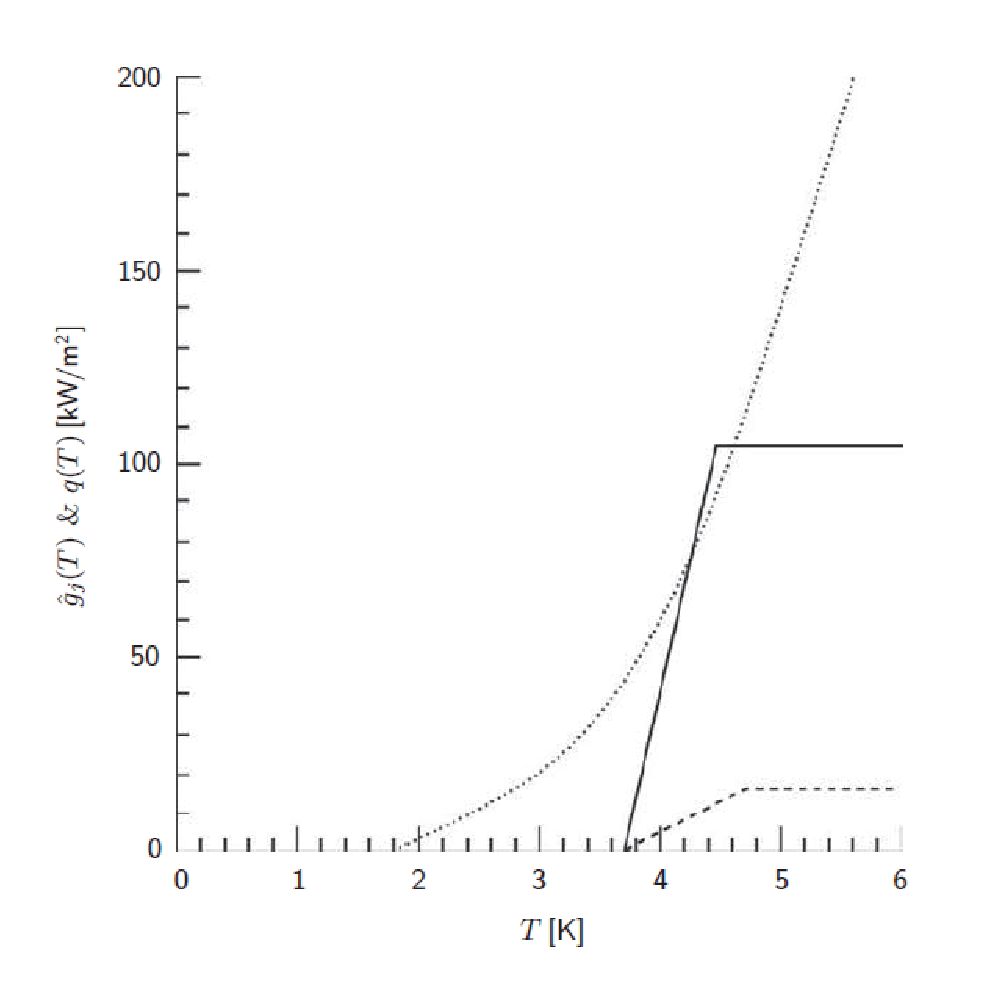
\includegraphics[scale=0.6]{chpt6/figs/fig6.19.eps}
	\caption{$\hat{g}_j(T)$(实线)和$q(T)$(点线);问题c)对应的$\hat{g}_j(T)$(虚线)。}
\end{figure}

c) $g_j(T)$和$q(T)$都和b)中计算的一样。本例中,相比没有隔层的绕组,单位导体长度暴露于液氦中的面积当然更大一些。
本例下,$f_p P_{cd}$ = (0.5)(23.6$\times 10^{-3}$ m) = 11.8$\times 10^{-3}$ m,以及$\hat{g}_j(T_c)$
= 9.34 $\mathrm{kW/m^2}$。

图6.19中的虚线给出了$\hat{g}_j(T_c)$图;用于前一个案例的$q(T)$仍然有效。
根据图,明显饼式线圈是低温稳定的。

\subsection{讨论6.7:低温稳定 vs 准绝热磁体}
如问题6.6所讨论的,混合III线圈的双饼在匝间没有冷却通道。
采用这种``准绝热"双饼的决策是为了减小应力。
使用术语``准绝热"是因为NbTi线圈在没有冷却通道的条件下不是低温稳定的,但近似于绝热工况的性能---随后,上述稳定性
分析作为一个练习给学生后,结果发现线圈是稳定的。
1986年FBML的一个内部研究(未公开发表)检验了机械扰动对线圈运行的影响,表明NbTi线圈在准绝热条件下将,也肯定会,有
令人满意的性能。

图6.20给出了一个NbTi导体制成的高场级(HF)和低场级(LF)低温稳定和准绝热绕组的
箍应力$\sigma_h$ vs. 线圈半径$r$的例子[3.14]。
对低温稳定绕组,因为有结构上的``软"匝间绝缘带,$\sigma_h$ vs. $r$与局部应力($r\times J\times B_z$)一致。
(HF-LF转变中的应力跳跃是因为导体截面的减小)
对准绝热绕组,因为绕组在径向更有刚性(无间隔垫片),内匝的径向膨胀由外部的绕组支撑,减小了内匝的应力。
净结果就是应力分布更加均匀。(分析中,假定了每部分的导体截面相同)
同等重要的是NbTi线圈总尺度的实质性减小,从外径1.06 m减小到约0.9 m。

\begin{figure}[htbp]
	\centering
	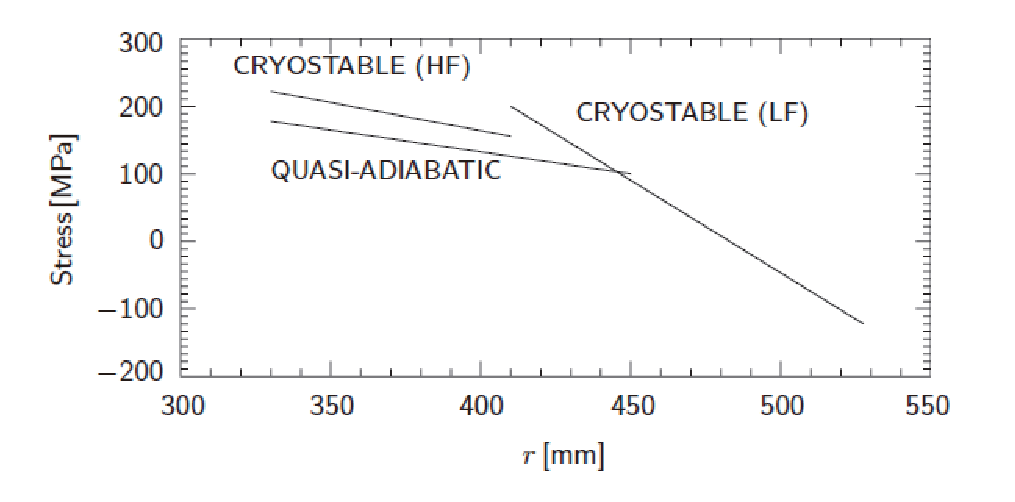
\includegraphics[scale=0.7]{chpt6/figs/fig6.20.eps}
	\caption{箍应力vs. 半径。}
\end{figure}


\subsection{讨论6.8:MPZ概念}
6.2.1部分简要的说明了MPZ概念在促进我们对发生于磁体绕组内部、影响几乎每一类磁体的``扰动"的理解的关键作用[1.27,6.14]。
这个表明降低LTS磁体性能的扰动的细微性[6.64,6.65]。

考虑一个无限半径的各向同性绕组(图6.21)运行在$I_{op}$,球形区域1($r\le R_{mz}$)全部是正常态,产生焦耳热密度
为$\rho_m J_m^2$,其中$\rho_m$是温度无关的基底电阻率,$J_m=I_{op}/A_m$;
区域2($r\ge R_{mz}$)是超导态;远离$R_{mz}$的区域,绕组温度是$T_{op}$。
假定绕组的热导率$k_{wd}$均匀且与温度无关,我们可以得到,在时不变和绝热工况下,除了焦耳热无其他耗散,
也即在方程6.1中,$C_{cd}\partial T/\partial t=0,g_d(t)=0,g_q(T)=0$。$R_{mz}$的表达式:
\begin{equation}% page391 第1个
R_{mz}=\sqrt{\frac{3k_{wd}(T_c-T_{op})}{\rho_mJ_m^2}}
\end{equation}

如果我们代入运行于液氦温度的LTS磁体的$k_{wd},T_c,T_{op},\rho_m,J_m$典型值,可以得到$R_{mz}$为0.1-10 mm。
(如果$k_{wd}$非各向同性,但正交各向异性,如实际绕组那样,MPZ的形状将变为椭球,而非球。)
相比于绕组体积,MPZ体积很小。但是,即使在绝热绕组中,它也可能有一个很小的$g_d(t)$,
它的大小程度需限制到$R_{mz}$之下。

\begin{figure}[htbp]
	\centering
	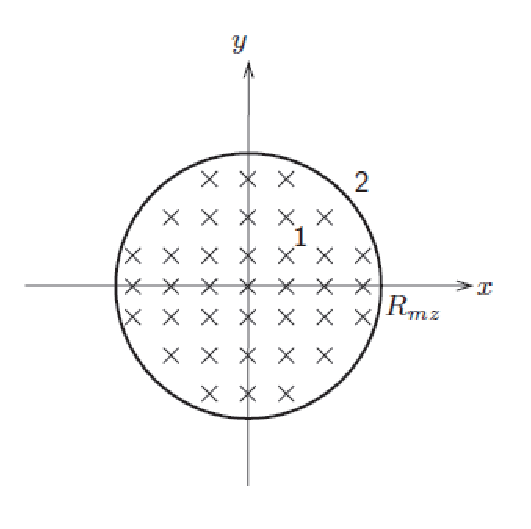
\includegraphics[scale=0.7]{chpt6/figs/fig6.21.eps}
	\caption{各向同性绕组。}
\end{figure}

尽管方程6.33中的$(T_c−T_{op})$在HTS绕组中要比LTS高一个数量级,
由于$\rho_m$随$T_{op}$增长而$k_{wd}$保持相对不变,在77.3 K时HTS绕组中的MPZ大小
差不多和运行于$T_{op}=4.2$ K的LTS磁体中的一样大。
一个对着运行温度显著增加的参数是绕组材料的焓密度。这样,如本章开始所述,由导线运动、环氧开裂等
机械事件产生的扰动能量几乎不可能让HTS磁体突破其临界温度。

\subsection{问题6.7:绝热绕组中的耗散能密度}
考虑一个无限长螺管线圈,内径$2a_1$,外径$2a_2$。
该磁体由制冷机冷却,在磁体周边(即内外径处)维持运行温度$T_{op}$,在绕组内部有一个均匀分布的耗散。
这个模型近似的是环氧浸渍绕组内的交流损耗被制冷机冷却的磁体。
在稳态条件下,绕组温度$T(r)$与时间无关,导体完全超导,即无焦耳损耗。应用于热各向同性绕组的功率密度是非常
简化的方程6.1:
\begin{equation}% page392 第1个
0=\nabla\cdot[k_{wd}(T)\nabla T]+g_d(t)
\end{equation}

式中,$k_{wd}(T)$是绕组的平均热导率。

a) 证明,在$k_{wd}(T)=k_{wd}$,为常数条件下,绕组温度$T(\rho)(1\le \rho\le\alpha,\rho\equiv r/a-1)$处在
空间均匀且恒定的热耗散密度$g_d(t)=g_d$下,可以写为:
\begin{equation}% page392 第2个
T(\rho)=\frac{a_1^2gd}{4k_{wd}}\left[(1-\rho^2)+(\frac{\alpha^2-1}{\ln \alpha})\ln\rho\right]+T_{op}
\end{equation}

b) 证明最大绕组温度$T_{mx}$出现在$\rho_{mx}$处:
\begin{equation}% page392 第3个
\rho_{mx}=\sqrt{\frac{\alpha^2-1}{2\ln \alpha}}
\end{equation}

c) 证明临界耗散密度$g_{d_c}$为下式。在该点的温升为绕组内最大,$\Delta T_{mx}\equiv T_{mx}-T_{op}$。
\begin{equation}% page392 第4个
g_{d_c}=\frac{4k_{wd}\Delta T_{mx}}{a_1^2\{1+\frac{\alpha^2-1}{2\ln \alpha}[\ln{(\frac{\alpha^2-1}{2\ln\alpha})}-1]\}}
\end{equation}
可见,$g_{d_c}$正比于$\Delta T_{mx}\equiv T_{mx}-T_{op}$。

我们可将上式写为:
\begin{align*}% page392 第5个
g_{dc}=\left(\frac{k_{wd}\Delta T_{mx}}{a_1^2}\right)\gamma_{d_c}(\alpha) \tag{6.37b}
\end{align*}

式中,无量纲参数为:
\begin{align*}% page392 第6个
\gamma_{d_c}(\alpha)\equiv\frac{4}{1+\frac{\alpha-1}{2\ln\alpha}[\ln(\frac{\alpha^2-1}{2\ln\alpha})-1]} \tag{6.37c}
\end{align*}

d) 画出方程6.37c给出的$\alpha$在1.25-5区间的$\gamma_{d_c}(\alpha)$。


\subsubsection{问题6.7之解}
a) 方程6.34在2D柱坐标中,令$k_{wd}(T)$为常数$k_{wd}$,有:
\begin{align*}% page393 第1个
\frac{k_{wd}}{r} \frac{d}{dr}(r\frac{dT}{dr})+g_d=0 \tag{S7.1a}
\end{align*}

代入$\rho\equiv r/a_1$,有:
\begin{align*}% page393 第2个
\frac{k_{wd}}{\rho}\frac{d}{d\rho}(\rho\frac{dT}{d\rho})+g_da_1^2=0 \tag{S7.1b}
\end{align*}

将上式对$\rho$积分两次,有:
\begin{align*}% page393 第3个
T(\rho)=-\frac{g_da_1^2}{4k_{wd}}\rho^2+A\ln\rho+B \tag{S7.2}
\end{align*}

加入边界条件$T(1)=T_{op}$和$T(\alpha)=T_{op}$,有:
\begin{align*}% page393 第4个
T(\rho)=-\frac{g_da_1^2}{4k_{wd}}[(1-\rho^2)+(\frac{\alpha-1}{\ln\alpha})\ln\rho]+T_{op} \tag{6.35}
\end{align*}

b) 将6.35对$\rho$微分,并令结果等于零,有:
\begin{align*}% page393 第5个
\frac{dT}{d\rho}=\frac{g_da_1^2}{4k_{wd}}[-2\rho+(\frac{\alpha^2-1}{\ln\alpha})\frac{1}{\rho}]=0 \tag{S7.3}
\end{align*}

解出$\rho$,有:
\begin{align*}% page393 第6个
\rho_{mx}=\sqrt{\frac{\alpha^2-1}{2\ln\alpha}} \tag{6.36}
\end{align*}

c) 在$\rho=\rho_{mx},T(\rho_{mx})=T_{mx}$时,根据方程6.35,有:
\begin{align*}% page393 第7个
T(\rho_{mx})\equiv T_{mx}=\frac{a_1^2g_d}{4k_{wd}}[(1-\rho_{mx}^2)+(\frac{\alpha^2-1}{\ln\alpha})\ln\rho_{mx}]+T_{op} \tag{S7.4}
\end{align*}

注意到在$T_{mx}$下,$\Delta T_{mx}=T_{mx}-T_{op}$和$g_d=g_{d_o}$。联立6.36和S7.4,有:
\begin{align*}% page393 第8个
\Delta T_{mx}=\frac{g_{d_c}a_1^2}{4k_{wd}}(1+\frac{\alpha^2-1}{2\ln\alpha}[\ln(\frac{\alpha^2-1}{2\ln\alpha})-1]) \tag{S7.5}
\end{align*}

解出:
\begin{align*}% page393 第9个
g_{d_c}=\frac{4k_{wd}\Delta T_{mx}}{a_1^2\{(1+\frac{\alpha^2-1}{2\ln\alpha}[\ln(\frac{\alpha^2-1}{2\ln\alpha})-)\}} \tag{6.37}
\end{align*}

d) 图6.22给出了$\alpha$在1.25-5区间的$\gamma_{d_c}(\alpha)$。
\begin{figure}[htbp]
	\centering
	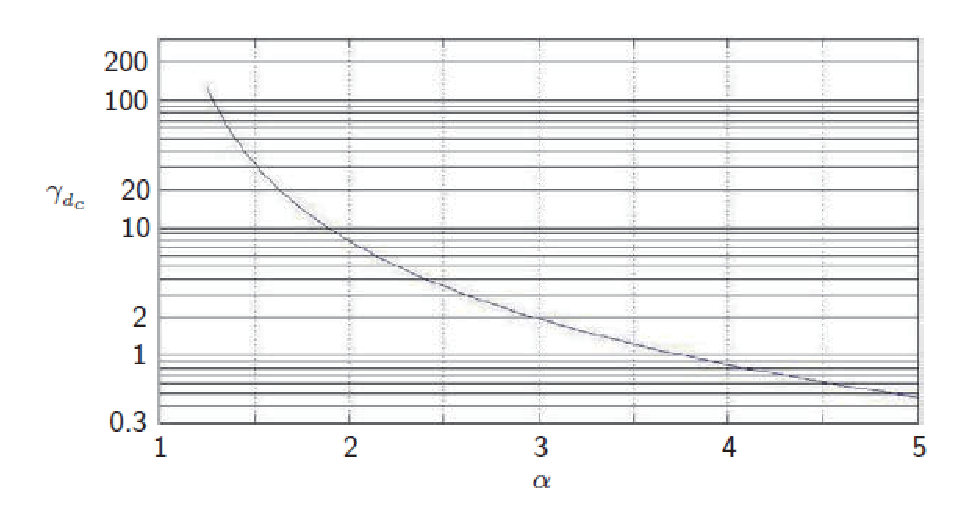
\includegraphics[scale=0.7]{chpt6/figs/fig6.22.eps}
	\caption{$\alpha$在1.25-5区间的$\gamma_{d_c}(\alpha)$}
\end{figure}

\textbf{实例}\quad 考虑几个可以近似实际案例的例子。

\textbf{例1:}\quad 这里我们考虑$\alpha=2;a_1$=10 cm;$k_{wd}=0.01\ \mathrm{W/cm K}$
(30 K的,由金属和绝缘组成的典型绕组);$\Delta T_{mx}$=3 K。
因为$\gamma_{d_c}(2)$=7.9,应用6.37b,有:
\begin{align*}% page394 第1个
g_{d_c}&=(\frac{k_{wd}\Delta T_{mx}}{a_1^2})\gamma_{d_c}(\alpha)\\\tag{6.37b}
&=\frac{(0.01\ \mathrm{W/cmK})(3\ \mathrm{K})}{(10\ \mathrm{cm})^2}(7.9)\simeq 2.4\times 10^{-3}\ \mathrm{W/cm^3}\simeq 2.4\times 10^3\ \mathrm{W/m^3}
\end{align*}

对这个$a_1$=10 cm和$a_2$=20 cm的轴向无限长HTS螺管,绕组温度维持在约30 K,由内外壁传导冷却,绕组内
有交流损耗等均匀耗散,在温度裕度$\Delta T_{mx}$至少为3 K时,
不破坏其超导性的最高能量密度为2.4 $\mathrm{kW/m^3}$。
这个耗散密度上限随$\Delta T_{mx}$增加而提高。
当然,尽管HTS可以在耗散密度2.4 $\mathrm{kW/m^3}$下保持全超导,但系统制冷负荷会变得非常重。

第七章将研究,一个宽为$w$,厚为$\delta$的HTS带,置于平行于带材宽度方向的周期磁场中,在多丝超导体中
占交流损耗三分之一的磁滞能量密度$e_{hy}\simeq\mu_0 J_c \delta H_m$,其中$J_c$是超导体的临界电流密度。
对YBCO带材,在30 K和2 T下,$J_c\simeq 2\times 10^9\ \mathrm{A/m^2},\delta\simeq 1\times 10^{-6}$ m;
这样,对$\mu_0 H_m=B_m=2$ T,我们有$e_{hy}=4\ \mathrm{kJ/m^3}$。
这个耗散能量密度等同于60 Hz下的240 $\mathrm{kW/m^3}$,是最大允许水平的100倍!
为了限制磁滞损耗能量密度到2.4 $\mathrm{kW/m^3}$,在相同的临界电流密度下,磁场必须小于0.02 T。注意,
这指的是平行于带材的磁场。


\textbf{例2:}\quad 此处我们考虑一个更薄的线圈:$\alpha=1.25$,其他参数相同。代入$\gamma_{d_c}(1.25)\simeq 128$,
有$g_{d_c}\simeq 38\ \mathrm{kW/m^3}$。

\textbf{例3:}\quad 对更厚的线圈,例如$\alpha=4,\gamma_{d_c}(4)\simeq 0.85$:
$g_{d_c}\simeq 260\ \mathrm{W/m^3}$。
这个临界耗散密度对HTS带材来说太低了---60 Hz的0.01 T的磁场下即有$1200\ \mathrm{W/m^3}$的磁能密度!
我们可以通过增强$k_{wd}$或将绕组分为薄壁线圈,各线圈分别内外壁冷却,以增加$g_{d_c}$,尽管明显需要增加制冷量。

\section*{参考文献}
\noindent [6.1] E.W. Collings, ``Design considerations for high Tc ceramic superconductors,” Cryogenics 28, 724 (1988).

\noindent [6.2] Y. Iwasa, ``Design and operational issues for 77-K superconducting magnets,” IEEE Trans. Mag. MAG-24, 1211 (1988).

\noindent [6.3] L. Ogasawara, ``Conductor design issues for oxide superconductors Part I: criteria of magnetic stability,” Cryogenics 29, 3 (1989).

\noindent [6.4] L. Dresner, ``Stability and protection of Ag/BSCCO magnets operated in the 20-40K range,” Cryogenics 33, 900 (1993).

\noindent [6.5] L.Y. Xiao, S. Han, L.Z. Lin, and H.M. Wen, ``Stability study on composite conductors for HTSC superconducting magnets,” Cryogenics 34, 785 (1994).

\noindent [6.6] J.W. Lue, L. Dresner, S.W. Schwenterly, D. Aized, J.M. Campbell, and R.E. Schwall, ``Stability measurements on a 1-T high temperature superconducting magnet,”
IEEE Appl. Superconduc. 5, 230 (1995).

\noindent [6.7] Yu. A. Ilyin, V.S. Vysotsky, T. Kiss, M. Takeo, H. Okamoto and F. Irie, ``Stability
and quench development study in small HTS magnet,” Cryogenics 41, 665 (2001).

\noindent [6.8] T. Obana, K. Tasaki, T. Kuriyama, and T. Okamura, ``Thermal stability analysis
of conduction-cooled HTS coil,” Cryogenics 43, 603 (2003).

\noindent [6.9] A.R. Kantrowitz and Z.J.J. Stekly, ``A new principle for the construction of stabilized superconducting coils,” Appl. Phys. Lett. 6, 56 (1965). Also see, Z.J.J. Stekly,
R. Thome, and B. Strauss, ``Principles of stability in cooled superconducting magnets,”
J. Appl. Phys. 40, 2238 (1969).

\noindent [6.10] J. Wong, D.F. Fairbanks, R.N. Randall, and W.L. Larson, ``Fully stabilized superconducting strip for the Argonne and Brookhaven bubble chambers,” J. Appl. Phys. 39, 2518 (1968).

\noindent [6.11] G. Bogner, C. Albrecht, R. Maier, and P. Parsch, ``Experiments on copper- and
aluminum-stabilized Nb-Ti superconductors in view of their application in large
magnets,” Proc. 2nd Int’l Cryo. Eng. Conf. (Iliffe Science and Technology Publication,
Surrey, 1968), 175.

\noindent [6.12] J.R. Purcell, ``The 1.8 tesla, 4.8m i.d. bubble chamber magnet,” Proc. 1968 Summer
Study on Superconducting Devices and Accelerators (Brookhaven National
Laboratory, Upton New York, 1969), 765.

\noindent [6.13] A.P. Martinelli and S.L. Wipf, ``Investigation of cryogenic stability and reliability
of operation of Nb3Sn coils in helium gas environment,” Proc. Appl. Superconduc.
Conf. (IEEE Pub. 72CHO682-5-TABSC), 331 (1977).

\noindent [6.14] L. Bottura \noindent [Private communication, 2004].

\noindent [6.15] B.J. Maddock, G.B. James, and W.T. Norris, ``Superconductive composites: heat
transfer and steady state stabilization,” Cryogenics 9, 261 (1969).

\noindent [6.16] M.N. Wilson and Y. Iwasa, ``Stability of superconductors against localized disturbances of limited magnitude,” Cryogenics 18, 17 (1978).

\noindent [6.17] J.E.C. Williams, E.S. Bobrov, Y. Iwasa, W.F.B. Punchard, J. Wrenn, A. Zhukovsky, ``NMR magnet technology at MIT,” IEEE Trans. Magn. 28, 627 (1992).

\noindent [6.18] Y. Iwasa and V.Y. Adzovie, ``The index number (n) below ‘critical’ current in
Nb-Ti superconductors,” IEEE Trans. Appl. Superconduc. 5, 3437 (1995).

\noindent [6.19] K. Yamafuji and T. Kiss, ``Current-voltage characteristics near the glass-liquid
transition in high-Tc superconductors,” Physica C 290, 9 (1997).

\noindent [6.20] Kohei Higashikawa, Taketsune Nakamura, Koji Shikimachi, Naoki Hirano, Shigeo Nagaya, Takenobu Kiss, and Masayoshi Inoue, ``Conceptual design of HTS coil for SMES using YBCO coated conductor,” IEEE Trans. Appl. Superconduc. 17, 1990
(2007).

\noindent [6.21] Mitchell O. Hoenig and D. Bruce Montgomery, ``Dense supercritical-helium cooled superconductors for large high field stabilized magnets,” IEEE Trans. Magn.MAG -11, 569 (1975).

\noindent [6.22] M. Morpurgo, ``A large superconducting dipole cooled by forced circulation of two phase helium,” Cryogenics 19, 411 (1979).

\noindent [6.23] P.J. Giarratano, V.D. Arp and R.V. Smith, ``Forced convection heat transfer to
supercritical helium,” Cryogenics 11, 385 (1971).

\noindent [6.24] Y. Iwasa, M.O. Hoenig, and D.B. Montgomery, ``Cryostability of a small superconducting coil wound with cabled hollow conductor,” IEEE Trans. Magn. MAG-13, 678 (1977).

\noindent [6.25] J.W. Lue, J.R. Miller, and L. Dresner, ``Stability of cable-in-conduit superconductors,” J. Appl. Phys. 51, 772 (1980).

\noindent [6.26] L. Bottura, ``Stability, protection and ac loss of cable-in-conduit conductors – a
designer’s approach,” Fusion Eng. and Design 20, 351 (1993).

\noindent [6.27] J.V. Minervini, M.M. Steeves, and M.O. Hoenig, ``Calorimetric measurement of
AC loss in ICCS conductors subjected to pulsed magnetic fields,” IEEE Trans.
Magn. MAG-23, 1363 (1980).

\noindent [6.28] T. Ando, K. Okuno, H. Nakajima, K. Yoshida, T. Hiyama, H. Tsuji, Y. Takahashi,
M. Nishi, E. Tada, K. Koizumi, T. Kato, M. Sugimoto, T. Isono, K. Kawano,
M. Konno, J. Yoshida, H. Ishida, E. Kawagoe, Y. Kamiyauchi, Y. Matsuzaki,
H. Shirakata, S. Shimamoto, ``Experimental results of the Nb3Sn demo poloidal
coil (DPC-EX),” IEEE Trans. Magn. 27 2060 (1991).

\noindent [6.29] G.B.J. Mulder, H.H.J. ten Kate, A. Nijhuis and L.J.M. van de Klundert, ``A new
test setup to measure the AC losses of the conductors for NET,” IEEE Trans.
Magn. 27, 2190 (1991).

\noindent [6.30] R. Bruzzese, S. Chiarelli, P. Gislon, and M. Spadoni, and S. Zannella, ``Critical
currents and AC losses on subsize cables of the NET-EM/LMI 40-kA Nb3Sn cablein-
conduit conductor prototype,” IEEE Trans. Magn. 27, 2198 (1991).

\noindent [6.31] D. Ciazynski, J.L. Duchateau, B. Turck, ``Theoretical and experimental approach
to AC losses in a 40 kA cable for NET,” IEEE Trans. Magn. 27, 2194 (1991).

\noindent [6.32] P. Bruzzone, L. Bottura, J. Eikelboom, A.J.M. Roovers, ``Critical currents and
AC losses on subsize cables of the NET-EM/LMI 40-kA Nb3Sn cable-in-conduit
conductor prototype,” IEEE Trans. Magn. 27, 2198 (1991).

\noindent [6.33] S.A. Egorov, A.Yu. Koretskij and E.R. Zapretilina, ``Interstrand coupling AC losses in multistage cable-in-conduit superconductors,” Cryogenics 32, 439 (1992).

\noindent [6.34] Naoyuki Amemiya, Takayuki Kikuchi, Tadayoshi Hanafusa and Osami Tsukamoto, ``Stability and AC loss of superconducting cables—Analysis of current imbalance and inter-strand coupling losses,” Cryogenics 34, 559 (1994).

\noindent [6.35] B.J.P. Baudouy, K. Bartholomew, J. Miller and S.W. Van Sciver, ``AC loss measurement of the 45-T hybrid/CIC conductor,” IEEE Trans. Appl. Superconduc. 5,
668 (1995).

\noindent [6.36] B. Blau, I. Rohleder, G. Vecsey, ``AC behaviour of full size, fusion dedicated cablein-conduit conductors in SULTAN III under applied pulsed field,” IEEE Trans.
Appl. Superconduc. 5, 697 (1995).

\noindent [6.37] Arend Nijhuis, Herman H.J. ten Kate, Pierluigi Bruzzone and Luca Bottura, ``First results of a parametric study on coupling loss in subsize NET/ITER Nb3Sn cabled specimen,” IEEE Trans. Appl. Superconduc. 5, 992 (1995).

\noindent [6.38] M. Ono, S. Hanawa, Y. Wachi, T. Hamajima, M. Yamaguchi, ``Influence of coupling current among superconducting strands on stability of cable-in-conduit conductor,” IEEE Trans. Magn. 32, 2842 (1996).

\noindent [6.39] K. Kwasnitza and St. Clerc, ``Coupling current loss reduction in cable-in-conduit
superconductors by thick chromium oxide coating,” Cryogenics 38, 305 (1998).

\noindent [6.40] Toshiyuki Mito, Kazuya Takahata, Akifumi Iwamoto, Ryuji Maekawa, Nagato
Yanagi, Takashi Satow, Osamu Motojima, Junya Yamamoto, EXSIV Group, Fumio
Sumiyoshi, Shuma Kawabata and Naoki Hirano, ``Extra AC losses for a CICC coil due to the non-uniform current distribution in the cable,” Cryogenics 38, 551 (1998).

\noindent [6.41] P.D.Weng, Y.F. Bi, Z.M. Chen, B.Z. Li and J. Fang, ``HT-7U TF and PF conductor
design,” Cryogenics 40, 531 (2000).

\noindent [6.42] Soren Prestemon, Stacy Sayre, Cesar Luongo and John Miller, ``Quench simulation of a CICC model coil subjected to longitudinal and transverse field pulses,”
Cryogenics 40, 511 (2000).

\noindent [6.43] Kazutaka Seo, Katuhiko Fukuhara and Mitsuru Hasegawa, ``Analyses for interstrand coupling loss in multi-strand superconducting cable with distributed resistance between strands,” Cryogenics 41, 511 (2001).

\noindent [6.44] Yoshikazu Takahashi, Kunihiro Matsui, Kenji Nishi, Norikiyo Koizumi, Yoshihiko Nunoya, Takaaki Isono, Toshinari Ando, Hiroshi Tsuji, Satoru Murase, and Susumu Shimamoto, ``AC loss measurement of 46 kA-13T Nb3Sn conductor for ITER,”
IEEE Trans. Appl. Superconduc. 11, 1546 (2001).

\noindent [6.45] Qiuliang Wang, Cheon Seong Yoon, Sungkeun Baang, Myungkyu Kim, Hyunki
Park, Yongjin Kim, Sangil Lee and Keeman Kim, ``AC losses and heat removal
in three-dimensional winding pack of Samsung superconducting test facility under
pulsed magnetic field operation,” Cryogenics 41, 253 (2001).

\noindent [6.46] S. Egorov, I. Rodin, A. Lancetov, A. Bursikov, M. Astrov, S. Fedotova, Ch. Weber,
and J. Kaugerts, ``AC loss and interstrand resistance measurement for NbTi cablein-
conduit conductor,” IEEE Trans. Appl. Superconduc. 12, 1607 (2002).

\noindent [6.47] A. Nijhuis, Yu. Ilyin, W. Abbas, B. ten Haken and H.H.J. ten Kate, ``Change of
interstrand contact resistance and coupling loss in various prototype ITER NbTi
conductors with transverse loading in the Twente Cryogenic Cable Press up to
40,000 cycles,” Cryogenics 44, 319 (2004).

\noindent [6.48] S. Lee, Y. Chu, W.H. Chung, S.J. Lee, S.M. Choi, S.H. Park, H. Yonekawa,
S.H. Baek, J.S. Kim, K.W. Cho, K.R. Park, B.S. Lim, Y.K. Oh, K. Kim, J.S. Bak,
and G.S. Lee, ``AC loss characteristics of the KSTAR CSMC estimated by pulse
test,” IEEE Trans. Appl. Superconduc. 16, 771 (2006).

\noindent [6.49] Y. Yagai, H. Sato, M. Tsuda, T. Hamajima, Y. Nunoya, Y. Takahashi, and
K. Okuno, ``Irregular loops with long time constants in CIC conductor,” IEEE
Trans. Appl. Superconduc. 16, 835 (2006).

\noindent [6.50] P. Bruzzone, B. Stepanov, R. Wesche, A. Portone, E. Salpietro, A. Vostner, and
A. della Corte, ``Test results of a small size CICC with advanced Nb3Sn strands,”
IEEE Trans. Appl. Superconduc. 16, 894 (2006).

\noindent [6.51] R.D. Blaugher, M.A. Janocko, P.W. Eckels, A. Patterson, J. Buttyan and E.J. Sestak, ``Experimental test and evaluation of the Nb3Sn joint and header region,”
IEEE Trans. Magn. MAG-17, 467 (1981).

\noindent [6.52] M.M. Steeves and M.O. Hoenig, ``Lap joint resistance of Nb3Sn cable terminations for the ICCS-HFTF 12 tesla coil program,” IEEE Trans. Magn. MAG-19, 378 (1983).

\noindent [6.53] A. Bonito Oliva, P. Fabbricatore, A. Martin, R. Museich, S. Patrone, R. Penco,
N. Valle, ``Development and tests of electrical joints and terminations for CICC
Nb3Sn, 12 tesla solenoid,” IEEE Trans. Appl. Superconduc. 3, 468 (1993).

\noindent [6.54] D. Ciazynski, B. Bertrand, P. Decool, A. Martinez, L. Bottura, ``Results of the
European study on conductor joints for ITER coils,” IEEE Trans. Magn. 32, 2332 (1996).

\noindent [6.55] P. Bruzzone, N. Mitchell, D. Ciazynski, Y. Takahashi, B. Smith, M. Zgekamskij,
``Design and R\&D results of the joints for the ITER conductor,” IEEE Trans. Appl. Superconduc. 7, 461 (1997).

\noindent [6.56] Philip C. Michael, Chen-Yu Gung, Raghavan Jayakumar, and Joseph V. Minervini, ``Qualification of joints for the inner module of the ITER CS model coil,” IEEE Trans. Appl. Superconduc. 9, 201 (1999).

\noindent [6.57] M.M. Steves, M. Takayasu, T.A. Painter, M.O. Hoenig, T. Kato, K. Okuno, H.
Nakajima, and H. Tsuji, ``Test results from the Nb3Sn US-demonstration poloidal
coil,” Adv. Cryo. Engr. 37A, 345 (1992).

\noindent [6.58] L. Krempasky and C. Schmidt, ``Theory of ‘supercurrents’ and their influence on
field quality and stability of superconducting magnets,” J. Appl. Phys. 78 5800 (1995).

\noindent [6.59] S. Jeong, J.H. Schultz, M. Takayasu, V. Vysotsky, P.C. Michael, W. Warnes, and
S. Shen, ``Ramp-rate limitation experiments using a hybrid superconducting cable,”
Cryogenics 36, 623 (1996).

\noindent [6.60] Vitaly S. Vysotsky, Makoto Takayasu, Sangkwon Jeong, Philip C. Michael, Joel
H. Schultz, and Joseph V. Minervini, ``Measurements of current distribution in a
12-strand Nb3Sn cable-in-conduit conductor,” Cryogenics 37, 431 (1997).

\noindent [6.61] N. Amemiya, ``Overview of current distribution and re-distribution in superconducting cables and their influence on stability,” Cryogenics 38, 545 (1998).

\noindent [6.62] Sangkwon Jeong, Seokho Kim and Tae Kuk Ko, ``Experimental investigation to
overcome the ramp-rate limitation of CICC superconducting magnet,” IEEE Trans.
Applied Superconduc. 11, 1689 (2001).

\noindent [6.63] Z.J.J. Stekly, ``Behavior of superconducting coil subjected to steady local heating
within the windings,” J. Appl. Phys. 37, 324 (1966).

\noindent [6.64] A.Vl. Gurevich and R.G Mints, ``Self-heating in normal metals and superconductors,” Rev. Mod. Phys. 59, 117 (1987).

\noindent [6.65] Michael J. Superczynski, ``Heat pulses required to quench a potted superconducting magnet,” IEEE Trans. Magn. MAG-15, 325 (1979).
